%%%%%%%%%%%%%%%%%%%%%%%%%%%%%%%%%%%%%%%%% 
% Masters/Doctoral Thesis 
%
% This template is based on a template by:
% Steve Gunn (http://users.ecs.soton.ac.uk/srg/softwaretools/document/templates/)
% Sunil Patel (http://www.sunilpatel.co.uk/thesis-template/)
%
% Template license:
% CC BY-NC-SA 3.0 (http://creativecommons.org/licenses/by-nc-sa/3.0/)
%
%%%%%%%%%%%%%%%%%%%%%%%%%%%%%%%%%%%%%%%%%

%----------------------------------------------------------------------------------------
%	PACKAGES AND OTHER DOCUMENT CONFIGURATIONS
%----------------------------------------------------------------------------------------

\documentclass[
12pt, % The default document font size, options: 10pt, 11pt, 12pt
%oneside, % Two side (alternating margins) for binding by default, uncomment to switch to one side
english, % ngerman for German
singlespacing, % Single line spacing, alternatives: onehalfspacing or doublespacing
%draft, % Uncomment to enable draft mode (no pictures, no links, overfull hboxes indicated)
%nolistspacing, % If the document is onehalfspacing or doublespacing, uncomment this  to set spacing in lists to single
%liststotoc, % Uncomment to add the list of figures/tables/etc to the table of contents
%toctotoc, % Uncomment to add the main table of contents to the table of contents
%parskip, % Uncomment to add space between paragraphs
%nohyperref, % Uncomment to not load the hyperref package
headsepline, % Uncomment to get a line under the header
%chapterinoneline, % Uncomment to place the chapter title next to the number on one line
%consistentlayout, % Uncomment to change the layout of the declaration, abstract and acknowledgements pages to match the default layout
]{MastersDoctoralThesis} % The class file specifying the document structure

\usepackage[utf8]{inputenc} % Required for inputting international characters
\usepackage[T1]{fontenc} % Output font encoding for international characters
\usepackage{stmaryrd}
\usepackage{mathpazo} % Use the Palatino font by default

\usepackage[font=itshape]{quoting} 
\usepackage[toc,page]{appendix}


\usepackage[nogin]{Sweave}
\usepackage{pdfpages}

\usepackage[backend=biber,style=numeric]{biblatex} % Use the bibtex backend with the authoryear citation style (which resembles APA)

\usepackage[activate={true,nocompatibility},final,tracking=true,kerning=true,spacing=true,factor=1100,stretch=10,shrink=10]{microtype}

\usepackage{eso-pic}
\newcommand\BackgroundPic{%
	\put(0,0){%
		\parbox[b][\paperheight]{\paperwidth}{%
			\vfill
			\centering
      % Indicar la imagen de fondo en el siguiente comando
			\includegraphics[width=\paperwidth,height=\paperheight,%
			keepaspectratio]{img/portada-ugr-sencilla}%
			\vfill
}}}

\addbibresource{./example.bib} % The filename of the bibliography

\usepackage[autostyle=true]{csquotes} % Required to generate language-dependent quotes in the bibliography

%----------------------------------------------------------------------------------------
%	MARGIN SETTINGS
%----------------------------------------------------------------------------------------

\geometry{
	paper=a4paper, % Change to letterpaper for US letter
	inner=2.5cm, % Inner margin
	outer=3.8cm, % Outer margin
	bindingoffset=.5cm, % Binding offset
	top=1.5cm, % Top margin
	bottom=1.5cm, % Bottom margin
	%showframe, % Uncomment to show how the type block is set on the page
}

%----------------------------------------------------------------------------------------
%	THESIS INFORMATION
%----------------------------------------------------------------------------------------

\thesistitle{The Satisfiability Problem} % Your thesis title, this is used in the title and abstract, print it elsewhere with \ttitle
\supervisor{Dr. Serafín Moral Callejón} % Your supervisor's name, this is used in the title page, print it elsewhere with \supname
\examiner{} % Your examiner's name, this is not currently used anywhere in the template, print it elsewhere with \examname
\degree{Computer Engineering and Mathematics} % Your degree name, this is used in the title page and abstract, print it elsewhere with \degreename
\author{Pedro Bonilla Nadal} % Your name, this is used in the title page and abstract, print it elsewhere with \authorname
\addresses{} % Your address, this is not currently used anywhere in the template, print it elsewhere with \addressname
\subject{Sciences} % Your subject area, this is not currently used anywhere in the template, print it elsewhere with \subjectname
\keywords{} % Keywords for your thesis, this is not currently used anywhere in the template, print it elsewhere with \keywordnames
\university{Universidad de Granada} % Your university's name and URL, this is used in the title page and abstract, print it elsewhere with \univname
\department{\href{https://decsai.ugr.es/}{Department of Computer Science and Artificial Inteligence}} % Your department's name and URL, this is used in the title page and abstract, print it elsewhere with \deptname
%\group{\ } % Your research group's name and URL, this is used in the title page, print it elsewhere with \groupname
\faculty{\href{http://faculty.university.com}{Faculty Name}} % Your faculty's name and URL, this is used in the title page and abstract, print it elsewhere with \facname

\AtBeginDocument{
\hypersetup{pdftitle=\ttitle} % Set the PDF's title to your title
\hypersetup{pdfauthor=\authorname} % Set the PDF's author to your name
\hypersetup{pdfkeywords=\keywordnames} % Set the PDF's keywords to your keywords
}

\newcommand{\miTitulo}{The SAT Problem\xspace}
\newcommand{\miNombre}{Pedro Bonilla Nadal\xspace}
\newcommand{\miGrado}{Doble Grado en Ingeniería Informática y Matemáticas}
\newcommand{\miFacultad}{Facultad de Ciencias\\
  Escuela Técnica Superior de Ingenierías Informática y de Telecomunicación}
\newcommand{\miUniversidad}{Universidad de Granada}
% Añadir tantos tutores como sea necesario separando cada uno de ellos
% mediante el comando `\\\medskip` y una línea en blanco
\newcommand{\miTutor}{
Serafín Moral Callejón \\ \emph{Ciencias de la Computación e Inteligencia Artificial}}
}
\newcommand{\miCurso}{2019-2020\xspace}


\usepackage[utf8]{inputenc}
\usepackage[spanish, british]{babel}
\usepackage{caption}
\usepackage{listings}
\usepackage{adjustbox}
\usepackage{enumitem}
\usepackage{boldline}
\usepackage{amssymb, amsmath}
\usepackage{amsthm}
\usepackage{soul}
\usepackage{upgreek}
\usepackage{wrapfig}
\usepackage{mathtools}
\usepackage{epigraph}

\usepackage{algorithm}
\usepackage[noend]{algpseudocode}

\usepackage{tikz} % Diagramas conmutativos.
\usetikzlibrary{positioning}
\usetikzlibrary{bayesnet}
\usetikzlibrary{babel}
\usetikzlibrary{automata}
\usetikzlibrary{trees}
\usepackage{xcolor}
\usepackage{soul}
\usepackage{graphicx}

\usepackage{enumitem}
\usepackage[dvipsnames]{xcolor}

\newtheorem{theorem}{Theorem}[section]
\newtheorem{corollary}{Corollary}[theorem]
\newtheorem{thesis}[theorem]{Thesis}
\newtheorem{lemma}[theorem]{Lemma}

\theoremstyle{definition}
\newtheorem{definition}{Definition}[section]
\newtheorem{proposition}{Proposition}[section]
\newtheorem{example}{Example}[section]
\newtheorem{remark}{Remark}[section]

\newcommand\myeq{\stackrel{\mathclap{\normalfont\mbox{?}}}{=}}

\definecolor{myred}{RGB}{128, 0, 0}
\definecolor{mycolor}{RGB}{0, 128, 0}

\usepackage[allcolors=myred]{hyperref}
\usepackage{mathrsfs}

\begin{document}

\frontmatter % Use roman page numbering style (i, ii, iii, iv...) for the pre-content pages

%\pagestyle{plain} % Default to the plain heading style until the thesis style is called for the body content



\includepdf{img/portada.pdf}

\cleardoublepage

% !TeX root = ../libro.tex
% !TeX encoding = utf8

%*******************************************************
% Little Dirty Titlepage
%*******************************************************

\thispagestyle{empty}

\begin{center}
  \large  

  \vspace*{\stretch{1}}

  \begingroup
  \huge{\miTitulo} \\ \bigskip
  \endgroup

  \textrm{\miNombre}

  \vspace{\stretch{5}}

\end{center}  

\newpage
\thispagestyle{empty}

\hfill

\vfill

\miNombre\ \textit{\miTitulo}.

Trabajo de fin de Grado.

Curso académico \miCurso.\\

\begin{minipage}[t]{0.25\textwidth}
  \flushleft
  \textbf{Responsable de tutorización}
\end{minipage}
\begin{minipage}[t]{0.40\textwidth}
  \flushleft
  \miTutor
\end{minipage}
\begin{minipage}[t]{0.35\textwidth}
  \flushright
  \miGrado
  \medskip

  \miFacultad
  \medskip

  \miUniversidad
\end{minipage}
\begin{flushleft}
\end{flushleft}

\endinput

% !TeX root = ../libro.tex
% !TeX encoding = utf8
%
%*******************************************************
% Declaración de originalidad
%*******************************************************

\thispagestyle{empty}

\hfill\vfill

\textsc{Declaración de originalidad}\\\bigskip

D.. \miNombre \\\medskip

Declaro explícitamente que el trabajo presentado como Trabajo de Fin de Grado (TFG), correspondiente al curso académico \miCurso, es original, entendida esta, en el sentido de que no ha utilizado para la elaboración del trabajo fuentes sin citarlas debidamente.
\medskip

En Granada a 29 de Junio de 2020.
\begin{flushleft} 
Fdo: \miNombre 

\end{flushleft}

\vfill

\cleardoublepage
\endinput

% !TeX root = ../libro.tex
% !TeX encoding = utf8

%*******************************************************
% Dedication
%*******************************************************
\thispagestyle{empty}
\phantomsection 
\pdfbookmark[1]{Dedicatoria}{Dedicatoria}

\hfill
\vfill

\begin{flushright}
\itshape
A Mariquilla, una constante positiva.
\end{flushright}

\vfill

\cleardoublepage
\endinput

\pagestyle{thesis}
{
  \hypersetup{hidelinks}
  \setcounter{tocdepth}{2}
  \tableofcontents

}



%*******************************************************
% Introducción
%*******************************************************

% \manualmark
% \markboth{\textsc{Introducción}}{\textsc{Introducción}} 
\chapter{Introduction}
Some 2300 years ago, in Greece,  the field of logic was discovered when some people start asking themselves about syllogisms. From that point on, the problem of satisfiability has been a central part of the science.  From my point of view, it is one of the most natural problem anyone could be asked,  Satisfiability is the study of what can be true under some free conditions.\\

It was not until the 20th century that this problem became something more than a philosophical question. The correct foundation has been laid by Bool and Lindenbaum. The mathematicians were moving from an understanding of science based on not-always-evident arguments to an axiomatized foundation. This shift in perspective became more intense when Hilbert gave some homework for the mathematical community at the beginning of the century. In particular, we are interested in Hilbert's second problem:


\begin{quoting}
Prove that the axioms of arithmetic are consistent. 
\end{quoting}

This interest in logic, as the tool that proves (at last) the mathematics to be perfectly formal was paired with the develop of one of the most influential revolution of the last century: the computation.\\

As the mid-century approached, while Gödel's second incompleteness theorem put a huge dump in the faith on axiomatism,  different theories were proposed with the aim of creating a thinking machine. It was Turing who finally got the right idea first (I don't know if Charles Babbage would agree with this statement). With the thinking/computing machine in place, it happened that this branch of the science was absorbed by mathematics, as every formal science that is incipient enough.  The idea of getting an automatic demonstrator based in the axioms hovered in the community.\\


Mathematicians wanted a theorem solver, and they dreamed about it in the form of a linear solver of first order logic formulas, that would solve them efficiently. It turns out that there was a much more problem underlying this apparent difficulty: the P vs NP.\\

The next big step forward was made in 1973 by Stephen Cook, as he proved that SAT problem was as least as difficult to solve as any other problem in NP, therefore, providing a simplification from NP $\subset^?$ P to  SAT $\in^? $ P. This theorem moved the emphasis in SAT from having a supportive role in the play of logic to be the main character of its own story.\\

As the century ended, the new homework for the community of mathematicians was not asked by another important enough mathematician. Instead, the mathematicians  were asked by the Clay Mathematics Institute, to solve the millennium problems. and one of them, as many already now, is whether NP $\subset^?$ P, that is, whether SAT$\in^?$ P. To this day no one truly know the answer. \\

Meanwhile, in the electronics engineering scene, more powerful computers were developed each day. As the computing power increased, computers enabled us to use them in other branches of science. A lot of this branches needed to solve problems at least as hard as SAT, that . Therefore, the community stated the search for a practical algorithm that  allows us to know whether or not something is satisfiable.\\


Since then, more sciences started to be interested in solving SAT. Nowadays, as John Franco and John Martin said:
\begin{quoting}
Satisfiability stands at the crossroads of logic, graph theory, computer science, computer engineering, and operations research.
\end{quoting}

I like to think about this crossroad as a bridge that everyone wants to cross for its results, but is guarded by both Mathematics and Computer Sciences, the rulers of Satisfiability solving.\\

This document attempts at giving an overview of some results in SAT solving complextity, as well as implementing some reductions to SAT solvers. \\

The first part, encompassed by chapters 1 to 3 is more theoretical and introduce the  the problem and describe the main open problems and hypothesis.
The second part, chapters 4 to 6, describe the most relevant algorithms, mainly in terms of asymptotic complexity. The third and  last part, chapter 7, we develop a library that allow us to elegantly solve some relevant NP-Complete problems, making use of cutting-edge solvers.\\


The main sources of this document were \cite{schoning2013satisfiability},\cite{marek2009introduction},\cite{arora2009computational} and \cite{imms-sat18}. The sources for each section and chapter are referenced within the text.

\section*{Main goals and results achieved}
The initials goals of this thesis were:
\begin{enumerate}
\item Accomplish a theoretical study of the complexity of SAT.
\item Study of reductions of mathematical problems to SAT.
\item Study the state-of-the-art of the algorithms solving SAT.
\item Study how can we solve MAXSAT using SAT and deduce theoretical complexity .
\end{enumerate}

The first three of the was completely successful. In the first part we study the complexity extensively, in the second part we study the algorithms as well as in the third part we make reductions. \\

The last one is a partial success result. We expose MAXSAT and present its complexity, we do not solve it by reducing it to SAT. The study of these reductions from MAXSAT to SAT is left as work to be done.\\

For the achievement of these goals, i have to make use of notions relating to: boolean algebra, computational models, probability,  graph theory, object oriented programming and software design.



\endinput
               

\begin{otherlanguage}{spanish}
  %*******************************************************
% Summary
%*******************************************************

\newpage



\chapter*{Summary}
\addcontentsline{toc}{chapter}{Summary}
\section*{Brief Summary}

On this Bachelors' Thesis we deepen our knowledge in the satisfiability problem for propositional logic. In order to do that we start from the understanding of logic and problems to the study of completeness in complexity classes. Is in this area where SAT is a cornerstone in the development of notion a new theories. When a theoretical understanding of the problem is achieve we proceed to look for efficient algorithms to solve it (SAT-Solvers or solvers). We consider both deterministics and probabilitics approaches to this task, and discuss their efficiency. We present the state of the art on solvers. To end this project we implement a library that use the notions explained thorough the text in order to solve some interesting math-related NP-Complete problems.\\

\textbf{keywords:} NP-Complete, SAT, QBF, Cook-Levin, DPLL, PPSZ.



\selectlanguage{spanish}
\section*{Resumen Extendido}

Durante la redacción de este trabajo estudiaremos un campo multidisciplinar que involucra, por lo general, tanto consideraciones propias de los intereses de las matemáticas como de los intereses del campo de la ingeniería informática. Por lo tanto, es difícil distinguir a grandes rasgos que partes son de mayor interés para un lector que pertenezca a solo una de las disciplinas. Sin embargo, intentaremos diferenciar en la medida de lo posible, que partes son de interés para cada una de estas materias. En caso de que esto no sea posible, justificaremos el interés que cada ciencia tiene.\\

La primera parte introduce el problema y estudia su complejidad. Procedemos a explicar que realizamos en cada capítulo.\\

\textbf{Capítulo 1:} En este capítulo exponemos los fundamentos de la lógica. El objetivo es introducir con la máxima formalidad posible el marco de trabajo durante todo el proyecto. 
Empezamos definiendo el Álgebra Booleana como un retículo distributivo. Posteriormente, demostramos el teorema de Knaster-Tarski para retículos completos. Definimos a continuación la Lógica Proposicional como un Lenguaje Formal. De este modo, primero especificamos la sintaxis y la semántica de este idioma. Definimos una semántica basada en asignaciones y asignaciones parciales. Consideramos que este capítulo suscita un interés principal en el campo de la matemática. Sin embargo, es recomendado que todo lector lo lea para poder comprender en toda su extensión los capítulos subsecuentes.\\

\textbf{Capítulo 2:} En este capítulo, definimos formalmente lo que es un problema e introducimos el problema SAT como un problema de decisión sobre el lenguaje de la lógica proposicional. Un  problema de decisión puede entenderse como un problema cuya respuesta es sí o no. La decisión que toma el problema SAT es decidir si una fórmula es satisfacible, esto es, si bajo alguna configuración de valores de verdad esta es cierta. Análogamente, definimos las variaciones de este problema que suscitan más interés, y que estudiaremos en el siguiente capítulo. Continuamos demostrando como se realiza un certificado de ejecución de SAT. Para ello demostramos la completitud de la regla de resolución. Por último, hablamos sobre los problemas de satisfacción de restricciones. Consideramos que la definición del problema es de interés para ambas disciplinas. La parte de completitud es más interesante para un punto de vista matemático, así como la última sección es más interesante para la ingeniería informática.\\

\textbf{Capítulo 3:} En la introducción hemos hablado del concepto de que todos los problemas de NP son como mucho tan difíciles como SAT. En este capítulo presentaremos formalmente este resultado y lo demostraremos. En la última sección estudiaremos algunas nociones aledañas a SAT en relación a la teoría de la complejidad.\\

Para poder introducir el problema introducimos los modelos de computación, que nos servirán como base para, una vez definidos los problemas, resolverlos. Estos modelos se basan en la noción de máquina de Turing. Sobre estos modelos creamos una división de los problemas basada en su dificultad, que son las clases de complejidad, y presentamos algunas de las más importante como P,NP o LSPACE. Llegados a este punto introducimos el problema P vs NP, junto con otros resultados y problemas abiertos de interés.\\


La tercera sección está destinada a introducir la teoría necesaria para enunciar y demostrar el teorema de Cook-Levin. Una vez realizado este teorema lo aprovechamos e  introducimos una serie de resultados análogos en las diferentes variaciones de SAT, presentadas en el capítulo previo. Este teorema nos habla de la dificultad de SAT relativa a otros problemas de NP. Reflexionamos sobre la posibilidad de que SAT pertenezca a P presentado la hipótesis ETH, una hipótesis tan ampliamente aceptada como no demostrada.En la última sección realizamos un desarrollo de teorías asociadas con el problema SAT. En particular, estudiamos la acción de grupos de permutaciones y negaciones sobre fórmulas CNF. Presentamos las asignaciones Autark así como su NP-Completitud,  desarrollamos el teorema de Tseitin que nos permita relacionar eficientemente SAT con GSAT, consideramos CoNP completitud y, para terminar, consideramos FSAT y la relación entre los métodos constructivos y no constructivos de resolución.\\

En relación a la división del trabajo en informática y matemáticas, consideramos que este capítulo debe ser de interés para ambas disciplinas. Proseguimos explicando la siguiente parte. En esta, nos centramos en los algoritmos de resolución. Dividimos nuestro estudio de los algoritmos en tres capítulos.\\


\textbf{Capítulo 4:} En este capítulo estudiamos los algoritmos de resolución sobre conjuntos restringidos de SAT donde se pueden conseguir mejores resoluciones. Empezamos considerando restricciones aplicando nociones de combinatoria. Esta sección es naturalmente para el lector informático. Entre los métodos destacamos para el lector matemático la aplicación que explicamos del Lema Local de Lovasz, asociando un grafo de adyacencia a cada fórmula para poder aplicar el resultado. Proseguimos explicando los famosos casos de 2SAT y HORNSAT. \\

\textbf{Capítulo 5:} En este capítulo estudiamos los algoritmos completos de resolución de SAT. Las dos estrategias principales estudiadas son el algoritmo DPLL. Este es un algoritmo que, sin tener una complejidad teórica mejor que los métodos más obvios, introduce un uso de heurísticas y los algoritmos basados en mejoras de este tiene un lugar muy relevante entre los casos prácticos de resolución de SAT. Entre sus mejoras mejoras incluimos el algoritmo de Monien-Speckenmeyer y la explicación de los muy extendidos algoritmos de Conflict-Driven-Clause-Learning.\\

Tomando otro enfoque explicamos el método de búsqueda local ajustado a SAT. Una vez descrito lo mejoramos aplicando la teoría de código de cubrimientos. Esta sección consideramos que tiene un interés natural para el ámbito de la ingeniería informática. Desde el ámbito de las matemáticas el interés reside en el análisis de la complejidad de los algoritmos.\\

\textbf{Capítulo 6:} En este capítulo realizamos un estudio profundo del probablemente campo más activo de los algoritmos SAT-solver: el campo de los algoritmos probabilísticos. En estos algoritmos hacemos un compromiso en el cual a cambio de ganar en eficiencia admitimos algoritmos con un error unilateral acotado, es decir, un algoritmo que siempre responda correctamente si una formula no es satisfacible, y tenga una probabilidad de responder correctamente si lo es. Entre los algoritmos probabilísticos, al igual que en la sección anterior estudiamos los dos enfoques: algoritmos basado en DPLL y algoritmos basados en busqueda Local. Entre los primeros estudiamos en profundidad el algoritmo PPZ y su mejora el algoritmos PPSZ. Este algoritmo es a día de hoy el que mejor eficiencia teórica presenta. En el ámbito de la búsqueda local encontramos el algoritmos de Schöning, que siendo uno de los más simples tiene una eficiencia no mucho peor a PPSZ. \\

Este capítulo es de interés para el ámbito de la informática debido al desarrollo de algoritmos de resolución. A su vez, un matemático puede ver reflejado sus intereses en la demostraciones realizadas para el estudio de la esperanza de error unilateral. Con esto acabamos la segunda parte.\\


\textbf{Capítulo 7:} Este capítulo, único perteneciente a la parte 3, narra el desarrollo de una biblioteca en Python basada en PySAT. El objetivo de esta biblioteca es realizar una resolución eficaz a la vez que elegante de problemas NP-Completos. Para esto realizamos reducciones de estos problemas al problema SAT. Esta biblioteca resuelve los problemas NP-Completos de Coloreado, Cubrimiento por grafos y existencia de camino hamiltoniano en grafos, así como el problema de distancia en cadenas. Por último desarrollamos naiveQBF que tiene como esperanza ser un esqueleto eficiente para el desarrollo de QBFsolvers basados en SAT. El código asociado a esta biblioteca esta disponible en:

\begin{center}
  \url{https://github.com/pedrobn23/TFG/}
\end{center}

El interés de esta sección para las matemáticas está en el desarrollo de herramientas para resolver problemas de su area de conocimiento. Para la informática está en las competencias demostradas en la organización, producción y acabado del código.\\

\textbf{palabras clave:} SAT, QBF, NP, NP-Completo, Cook-Levin, DPLL.


\selectlanguage{english}


% \endinput
                    
\end{otherlanguage}






\mainmatter % Begin numeric (1,2,3...) page numbering

 % Return the page headers back to the "thesis" style

% Include the chapters of the thesis as separate files from the Chapters folder
% Uncomment the lines as you write the chapters

% Chapter 1

\part{Satisfiability Problem: Definition and Relevance} % Main chapter title

\label{Chapter1} % For referencing the chapter elsewhere, use \ref{Chapter1} 

% ----------------------------------------------------------------------------------------

% Define some commands to keep the formatting separated from the content 
\newcommand{\keyword}[1]{\textbf{#1}}
\newcommand{\tabhead}[1]{\textbf{#1}}
\newcommand{\code}[1]{\texttt{#1}}
\newcommand{\file}[1]{\texttt{\bfseries#1}}
\newcommand{\option}[1]{\texttt{\itshape#1}}

% ----------------------------------------------------------------------------------------

\chapter{Logic}

\begin{itemize}
\item[TODO:]$\qquad$ Incluir introducción del problema.

\item[INFO:]
  \begin{itemize}
  \item Explicar que vamos a explicar en este capítulo.
  \item Handbook incluye una introducción histórica.
  \item Libro verde incluye una introducción intuitiva excelente.
\end{itemize}
\end{itemize}


In this chapter we present the bases of Logic and formal languages. Logic will provide us with a framework on which we will be able to define the Satisfiability Problem. We will present the area with formality, explaining only the things that will be necessary for our goal.


\section{Boolean Algebra}

The same way I started my journey on the university, we could have started this text right from the axioms, making a really romantic thesis. Nonetheless, given the goal we want to achieve, it seems excessive. We will refer to the commonly used \emph{Zermelo-Fraenkel axioms}, in order to have a point of reference, and therefore we will work without more considerations with sets and set operations. We will only be concerned with finite sets for most cases.\\

Further on this section we will present Boolean Algebra in a classic lattice-based way that could be found in related literature. In particular we follow  \emph{Introduction to mathematics of satisfiability}\cite{marek2009introduction} for the definition of boolean algebra and propositional logic. The definition of Lattice of Partitions is adapted from \cite{sakallah2009symmetry}

\begin{definition}
  A partial ordered set, also poset, is a pair $\{X, \le\}$ where $X$ is a set and $\le$ is a partial order of $X$. A chain $Y$ of $\{X, \le\}$ is a subset of $X$ where $\le$ is a total order. 
\end{definition}



\begin{definition} A lattice is a partial ordered set 
$ \{X,\le\} $ where every pair of elements possesses a least upper bound and a greatest lower bound. A lattice has two new operations defined: given two elements $x,y\in X$
  \begin{itemize}
  \item $x\vee y$ denote the least upper bound.
  \item $x\wedge y$  denote the greatest lower bound.
  \end{itemize}
\end{definition}


  A lattice is complete if every subset has an unique largest element and an unique lowest element. A lattice is presented generally as a duple $\{L,\le\}$, a triple $\{X,\vee,\wedge\}$ and, whenever possible, is presented as a quintuple $\{X, \vee, \wedge, \top,\bot\}$ where $\top$ is the greatest element and $\bot$ the lowest element. A lattice is called distributive if $x\vee(y \wedge z) = (x\vee y) \wedge (x \vee z)$ and $x\wedge(y \vee z) = (x\wedge y) \vee (x \wedge z)$



With the concept of lattice just included, we present the \emph{Knaster and Tarski fixpoint theorem}. In order to do that we will introduce some concepts. Given a function $f:\{L,\le\}\to \{L,\le\}$, a prefixpoint (resp. postfixpoint) is a point $x \in L$ such that $f(x) \le x$ (resp. $f(x) \ge x$). A fixpoint is a point that is both prefixpoint and postfixpoint. Note that, given that they exists, $\top$ and $\bot$ are a prefixpoint and a postfixpoint of $f$ respectively.

\begin{theorem}[Knaster and Tarski fixpoint theorem \cite{marek2009introduction}]
  \label{the:fixpoint}
  Let $f:\{L,\le\}\to \{L,\le\}$ be a monotone function in a complete lattice. Then:
  \begin{enumerate}
  \item $f$ has a least prefixpoint $l$ that is a fixpoint.
  \item $f$ has a largest postfixpoint $l$ that is a fixpoint.
  \end{enumerate}
\end{theorem}
\begin{proof}\hfill  \begin{enumerate}
  \item We know that there is at least a prefixpoint. Let
    $$l = \bigwedge_{\{x\in X: x\text{ is a prefixpoint}\}} x .$$ 
    Lets prove that $l$ is a fixpoint. Le $x$ be an arbitrary fixpoint, therefore, $l \le x \le f(x)$. Since $x$ was arbitrary, $f(l) \le l$. To show that it a fixpoint it suffices to see that $f(l)$ is a prefixpoint to, as $f$ is monotone.
  \item Apply the previous result on $f:\{L,\le\}\to \{L,\le\}$.
  \end{enumerate}
\end{proof}


\begin{definition}
  A \emph{Boolean algebra} is a distributive lattice  $\{X, \vee, \wedge, \top,\bot\}$ with an additional operation $\neg$, called complement or negation, such that for all $x\in X$:
  \begin{enumerate}
  \item $ x\wedge \neg x = \bot,\ x\vee \neg x = \top $.
  \item $ \neg(x \vee y) = \neg x \wedge \neg y,  \neg(x \wedge y) = \neg x \vee \neg y$.
  \item $\neg \neg x = x$.
  \end{enumerate}
\end{definition}




\begin{definition}[Lattice of Partitions]
Given a set $X\ne \emptyset$, we denote as $\mathcal{P}(X)$ the partitions of $X$. Let $\pi,\pi'\in \mathcal{P}(X)$. We say that $\pi\le_{\mathcal{P}}\pi'$ if for every $A\in \pi$ there exists $B\in \pi'$ such that $A\subset B$. The \emph{lattice of partitions} of $X$ is the lattice $\{\mathcal{P}(X),\le_{\mathcal{P}}\}$.
\end{definition}

For example given the lattice $\{\mathcal{P}(\{1,2,3,4\}),\le_{\mathcal{P}}\}$ and two partitions:

\begin{equation}
    \begin{split}
      \pi_1 & = \{\{1,2\},\{3,4\}\}\\
      \pi_2 & = \{\{1,2,3\},\{4\}\}
\end{split}
\end{equation}

We have that:
\begin{equation}
    \begin{split}
      \pi_1\land\pi_2 & = \{\{1,2\},\{3\},\{4\}\}\\
      \pi_1\lor\pi_2 & = \{\{1,2,3,4\}\}
\end{split}
\end{equation}

  
\section{Propositional Logic}
Propositional logic is the framework that will allow us define the main topics of this text.  Let's define some concepts:
\begin{itemize}
\item An alphabet $A$ is an arbitrary finite non-empty set.
\item A symbol $a$ is an element of the alphabet.
\item A word $w = \{a_i:i\in 1,..,n\}$ is a finite sequence of symbols.
\item The collection of all possible words over an alphabet $A$ is denoted by $A^*$.
\item A language $L$ over $A$ is a subset of $A^*$.
\end{itemize}

For example, Spanish is a language with a well-known alphabet. Also, Spanish is a proper language over its alphabet as it is not empty, and it does not include all possible words.\\

When we talk about a logic system we are talking about a distinguished formal language. A formal language is defined by it syntax and its semantics. The syntax is the rules that define the language. They state what words over an alphabet are valid in the language. The semantics deal with the interpretations of the elements in the language. Usually this is achieved by assigning truth values to each word.\\

We will define now propositional logic, or zeroth-order-logic. \\

\begin{figure}[h]
  \begin{center}
    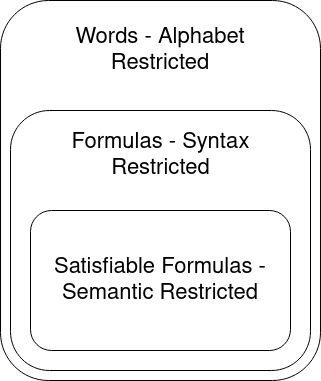
\includegraphics[width=5cm]{/home/pedro/Carrera/Quinto/TFG/tesis/figures/sintax2.png}
    \caption{Diagram showing the different classes which are constructed on the formal language of Propositional Logic.}
  \end{center}
\end{figure} 

\subsection{Syntax of Propositional Logic}
We first start with the basic building blocks, which collectively form what is called the alphabet:
\begin{itemize}
\item Symbols $x,y,z$ for variables. As more variables are necessary sub-indexes will be used.
\item Unary operator $\neg$ (negation). A literal will refer to a variable or a negated variable. Thorough the text symbol $l$ will denote a literal. 
  
\item Values 0 and 1. These values are often named as $\bot$ and $\top$ respectively.

\item Binary operators: $\wedge, \vee, \rightarrow, \oplus, \iff $
\end{itemize}


The words of Propositional Logic are called formulas.
\begin{definition}
  A Boolean formula is defined inductively:
  \begin{itemize}
  \item The constants 0 and 1 are formulas.
  \item Every variable is a formula.
  \item If $F$ is a formula, then $\neg  F$ is a formula.
  \item The concatenation with a binary operator of two formulas is a formula too.\\
  \end{itemize}
\end{definition}

Examples of formulas are $x\vee y$ or $x_1\wedge x_2 \vee  ( x_4 \vee \neg  x_3 \wedge (x_5\to x_6) \vee 0 )$.We should distinguish a special type of formula: the clauses. A clause  is a formula with the form $l_1\vee ... \vee l_n$ where $l_i, i \in 1,...,n$ are literals. Clauses are will be often regarded as a finite set of literals. Example of a clause is $(x_1\vee \neg x_4 \vee x_2)$. When regarded as a set every clause $C$ has a cardinal $|C|$, that represents the number of literals contained. \\


  We will denote by $Form$ the set of all formulas. We define a special mapping, $Var$, that assigns every formula to its variables. Furthermore, for a given set of variables $X$ we define $Form_{X}$ as the set of all formulas that can be constructed from $X$. The reader should note that $Form_X = Var^{-1}(X)$.


\subsection{Semantics of Propositional Logic}
The underlying problem of semantics is to develop methods to give meaning to the elements allowed by the syntax.When facing a way to provide semantic meaning to formulas the use of function In this section we will discuss to ways of providing meaning to the formulas: two-valued logic and three valued logic.\\ 



In two valued logic define the truth value of a formula by assigning a truth value(1 for Truth and 0 for False) to each variable. Note that we assign a meaning of truth to the constants 1 and 0, that until now where meaningless. The truth value of the formulas that involve operators are provide by their truth table.


\begin{table}[h]
  \begin{center}
    \begin{tabular}{|l|l|l|l|l|l|l|l|}
      \hline
      $p$ & $q$ & $\neg p$& $p\vee q$ & $p\wedge q$ & $p \oplus q$ & $p \to q $ & $p \iff q$  \\ 
      \hline
      0 & 0 & 1 & 0 & 0 & 0 & 1&1\\
      0 & 1 & 1 & 1 & 0 & 1 & 1&0\\
      1 & 0 & 0 & 1 & 0 & 1 & 0&0\\
      1 & 1 & 0 & 1 & 1 & 0 & 1&1\\\hline
    \end{tabular}
  \end{center}
  \caption{\label{tab:table-name}Truth tables of different operators in two valued logic.}
\end{table}


The truth value of a formula is therefore obtained by replacing each variable by their assigned constant and propagating the value. The tool that we will use to assign a truth value to each variable is the assignments.

\begin{definition}
  Let $X$ be a finite set of variables. An assignment is a function $\alpha$ from $Form_X$ to $Form_X$, on which some variables $\{x_1,...,x_n \}$ are replaced by predefined constants $\{a_1,...,a_n\}$ respectively.\\
\end{definition}

An assignment that assigns a value to a variable $x$ is said to map the variable $x$. In two valued logic we will consider only assignment that maps all variables, and therefore all formulas are given a value by an assignment. We also see that any assignment generate a map from $X$ to $\{0,1\}$. Conversely, any map from $X$ to $\{0,1\}$ would uniquely represent a assignment $alpha$ over $Form$. In practice when we talk about an assignment $\alpha$ we will refer indistinctly to either the function over $Form_{Var}$ or the mapping  over $Var$.\\

One can then \emph{apply} an assignment $\alpha$ to a formula $F$, denoting it by $F\alpha=\alpha(F)$. To describe an assignment we will use a set that pairs each variable to it value, i.e. $\alpha=\{x_1\to 1,...,x_n\to 0\}$. For example given an assignment $\alpha_0 = \{x_1 \to 1, x_2\to 1, x_3 \to 0, x_4 \to 1\}$ and $F_0=x_1\to (x_2\wedge x_4)$ then  $F_0\alpha_0=1 \to (1\wedge 1)= 1$. \\    

\begin{definition}
  An assignment is said to \emph{satisfy}  a formula $F$ if $F\alpha=1$ and in the case $F  \alpha = 0 $ it is said to \emph{falsify} the statement. A formula $F$ is called \emph{satisfiable} if is exists an assignment that satisfies it. Otherwise it is called \emph{unsatisfiable}.
\end{definition}


Note that we have a really restrictive constraint on assignments: they should map all variables.  This is so in order for an assignment to give a meaning to every formula. To ease this constraint we use three-valued logic. On three valued logic we have three significant: True or 1, False or 0, and unknown or $\upsilon$. Now the assignment will map every variable to one of these values. These new assignments will be called partial assignments, as they only map some variables to a truth value. We can propagate the previous values adding new rules.

\begin{table}[h]
  \begin{center}
    \begin{tabular}{|l|l|l|l|l|l|l|l|}
      \hline
      $p$ & $q$ & $\neg p$& $p\vee q$ & $p\wedge q$ & $p \oplus q$ & $p \to q $  & $p \iff q$  \\ 
      \hline
      
      $\upsilon$ & 0 & $\upsilon$ & $\upsilon$ & 0 & $\upsilon$ & $\upsilon$ & $\upsilon$\\
      $\upsilon$ & 1 & $\upsilon$ & 1 & $\upsilon$ & $\upsilon$ & 1 &$\upsilon$\\
      0 & $\upsilon$ & 1 & $\upsilon$ & 0 & $\upsilon$ & 1 &$\upsilon$\\
      1 & $\upsilon$ & 0 & 1 & $\upsilon$ & $\upsilon$ & $\upsilon$ &$\upsilon$\\
      \hline

    \end{tabular}
  \end{center}
  \caption{\label{tab:table-name}Truth table of different operators in three valued logic.}
\end{table}


In practice partial assignments will be only defined by denoting only the variables that are mapped to either 0 or 1. We can see that the composition of assignments (seen as functions over $Form_{var}$) is also a partial assignment. Also, when applying a partial assignment to a formula, instead of mapping it to $\upsilon$ we will avoid operating over the variables assigned to $\upsilon$. For example given a partial assignment $\alpha_0 = \{x_1 \to 1, x_2\to 1, x_3 \to 0\}$ and $F_0=x_1\to (x_2\wedge x_4)$ then  $F_0\alpha_0=1 \to (1\wedge x_4)= 1 \to (x_4)$. Although $F_0$ is mapped to another formula by $\alpha_0$, $\alpha_0$ is still providing a meaning to it (the unknown meaning). \\



Partial assignments will be also used to iteratively \emph{expand} them: let $Var= \{x_i:i\in 1,...,n\}$ the set of variables and let $\alpha_1$ be partial assignment that map variables $[x_1\to a_1,...,x_j\to a_j]$ with $1<j<n$ and $a_j\in\{0,1\}$ for every $j$, we can expand it by choosing a nonempty subset  $A\subset\{a_k: k\in j+1,..,n\}$ and a value $c_x \in \{0,1\}$ for every $x\in A$. Then we can define:

$$
\alpha_2(x)=
\begin{cases}
  \alpha_1(x) & x \in \{x_i : i \in 1,...,n\},\\
  c_x & x\in A, \\
  \upsilon & \text{otherwise}.
\end{cases}
$$

We can see that $\alpha_2$ expands $\alpha_1$ in the sense that the truth value assigned to a formula by $\alpha_1$ holds in $\alpha_2$ if it were different that unknown. Therefore we are expanding the 'known' values of the formulas. Note that in the definition of $\alpha_1$ it were not necessary to state what variables were mapped to $\upsilon$ at it was implicit that every variable not listed were of unknown  value.\\

In practice we will try to avoid refer to this process whenever is evidently enough what is being done. Nonetheless partial assignments will be a central part of algorithms such as DPLL[\ref{sec:dpll}]. When context is clear enough, assignments will be used for both assignments and partial assignments.\\

Arguably, the most special case of partial assignment are autarks assignments[\ref{sec:autark}]. An autark assignment is a partial assignment that simplify a formula in a sense latter explained.\\

Given an assignment or partial assignment $\alpha$ we will denote the set of variables mapped to either 0 or 1 by $Var(\alpha)$. Analogously, given a formula $F$, $Var(F)$ will denote the variables that appear in $F$. Note that if $F\in Form_{Var}$ then $Var(F)\in Var$ and it is not necessary that $Var(F)=Var$.\\

Naturally, we want theorems to be the formulas that are always true. In the context of propositional logic, theorems are the tautologies.   

  \begin{definition}
    Let $X$ be a set of variables. A formula $F\in Form_X$ is a \emph{tautology} if for every two-valued assignment $\alpha$ over $X$ we have that $F\alpha=1$. We say that $G$ \emph{follows from} $F$ if $F\to G$ is a tautology. 
  \end{definition}


  
Two formulas $F,G$ are said to be equal, represented as $F\sim G$, if for every two-valued assignment $\alpha$ we have $F\alpha = G\alpha$. It follows from the equivalently properties on constants that $\sim$ is an equal relationship. This definition is really intuitive, as it defines as equal the formulas that has the same meaning in every possible situation. Note that this definition is equivalent to ensure that both $F\to G$ and $G\to F$ are tautologies.\\



\label{def:linden}
With $\sim$ defined we can have what is called a \emph{Lindenbaum algebra}, as a quotient space of $Form = Form_{Var}$ by the relation $\sim$, denoted as $Form/\sim$. It follows that every operator respect the quotient space structure, i.e., for every $[\phi_1],[\phi_2]\in\ Form/\sim$:

\begin{itemize}
\item $\neg [\phi_1] = [\neg\phi_1]$
\item $ [\phi_1] \vee [\phi_2]= [\phi_1 \vee \phi_2]$
\item $ [\phi_1] \wedge [\phi_2]= [\phi_1 \wedge \phi_2]$
\end{itemize}

The interest of Lindenbaum algebra resides in the fact that $\{Form/\sim, \vee,\wedge,[1],[0]\}$ is a Boolean algebra, providing therefore a nexus between the algebraic formulation of the problem an its semantics.










\chapter{Definition of the problem}
\section{Satisfiability Problem}
\subsection{Decision Problems}
Computability and complexity theory attempts to answer questions regarding how to solve real-world problems efficiently. In this subsection we provide a formal approach to the concept of problem, and its resolution.\\

We will study the complexity of functions. In order to standardize the approach we code the input of the function and the output of the functions using words over a finite alphabet. As for every finite alphabet $A$ there is a bijective mapping from $A^*$ to $\{0,1\}^*$ we can assume when it is convenient that the alphabet is $\{0,1\}$. With this convention we are now ready to define what a decision problem is.

\begin{definition}[Decision Problem\cite{arora2009computational}]
  Given a language $L$ over an alphabet $A$, it has an associated decision problem that consists on, given a word $w\in A^*$ check whether $w$ is in $L$. 	
\end{definition}


When we have a named language, we refer indistinctly by this name to both the language and the associated decision problem. In order to define a decision problem it is only needed to define a language over an alphabet. Therefore a decision problem may be defined implicitly, that is, as the set of the words in an alphabet that satisfy some condition. As semantics provides meaning to the languages, real world problems can be addressed as decision problems.\\

As a last definition of this subsection, we introduce the complement decision problem.
\begin{definition}[Complement Decision Problem\cite{arora2009computational}]\label{def:complement}
  Given a decision problem  $L$ it has a Complement Decision Problem named $CoL$ that consists on, given a word $w\in A^*$ check whether $w$ is in $L$. 	
\end{definition}

This definition will be used further in [\ref{sub:detcomp}] in order to define complexity classes.


\subsection{Definition}

Given the previous definitions, we are now almost prepared to define the central part of this thesis: the satisfiability decision problem of propositional logic, SAT for short. To this end we define a special subset of formulas in Propositional Logic: the formulas in Conjunctive Normal Form.

\begin{definition}
  A formula $F$ is said to be in Conjunctive Normal Form ($CNF$) if $F$ is written as:x
  $$F = C_1\wedge ... \wedge C_n.$$
  Where $C_i$  are clauses.
\end{definition}

Note that every formula in $CNF$ can be regarded as a set of clauses. This approach is really useful in some contexts and will be used continuously on this text.

\begin{definition}
  The Satisfiability Language of Propositional Logic (SAT) is the language over the alphabet of propositional logic that includes all formulas that are both satisfiable and in $CNF$.
\end{definition}

We will refer with the acronym $SAT$ to both the language and the associated decision problem. As checking if a formula is in CNF is a fairly simple syntax problem, we are only interested in asserting whether or not a formula in $CNF$ is satisfiable.

\begin{definition}
  A \emph{SAT-Solver} is an algorithm that, being given a formula $F$ in \emph{CNF} as input, answer whether or not is satisfiable.
\end{definition}

On chapter[\ref{chap:2}] we analyze the main SAT-solver developed in the literature. We will differentiate two types of SAT-Solver. The algorithms that, given enough time always output the correct result at the end are called \emph{complete}. The SAT-solvers that doesn't guaranty its result are called \emph{incomplete}. Of particular interest among incomplete SAT-solvers are the one-sided bounded error SAT-solvers. These are the called probabilistic algorithms, discussed on Section \ref{sec:prob}.


\section{Variations}

The SAT decision problem quite a lot of variations, all of them of interest for certain complexity classes. We will list some of the most important, starting with two decision problems. The first of them is a natural generalization.

\begin{definition}
  The Generalized Satisfiability Language of Propositional Logic (GSAT) is the language over the alphabet of propositional logic that includes all formulas that are Satisfiable.
\end{definition}

With Tseitin's Theorem[\ref{the:Tseitin}] we can see that these two problems are in fact fairly similar. More often than not GSAT will be solved by solving an equivalent SAT problem. Analogously a \emph{GSAT-Solver}  is a SAT-solver that also accepts as inputs formulas not in CNF. Further on, every new problem will have a associated \emph{solver}, defined analogously.



\begin{definition}
  Let $F$ be a formula. $F$ is said to be $k$-CNF formula (equivalently a formula in $k$-CNF) if it is in CNF and $\forall C \in F, |C| = k$. $k$-SAT is the language of the formulas that are both satisfiable and in $k$-CNF.
\end{definition}

Other variations of SAT could be achieved by generalizing the concept of decision problem.

\begin{definition}[Function Problem]
  Let $A,B$ be two sets. Given a relation $R\subset A\times B$, it has an associated function problem that consists on, given a word $a\in X$ find a word $b\in B$ such that $(a,b)\in R$.
\end{definition}

We can consider decisions problems as a particular subset of function problems: Given a language $L\subset A^*$ we define the relationship $R\subset A^*\times \{0,1\}$ such that $(x,1)\in R$ iff $x\in L$ and $(x,0)\in R$ otherwise.history of the cook theorem   

\begin{definition}
  Let $CNF$ be the set of propositional formulas in CNF and $B$ the set of assignments.  The Satisfiability Function Problem of Propositional Logic (FSAT) is the function problem defined by the relation $$R=\{(F, b): F\in CNF, b \in B, Fb = 1\}.$$
\end{definition}
That is, is the problem of finding an assignment that satisfy a formula. Most of SAT-solvers not only try to solve SAT but also to solve FSAT, i.e., try to find an assignment that satisfy  the formula should it exists.
\begin{definition}
  Let $CNF$ be the set of propositional formulas in CNF and $B$ the set of assignments. The Maximum Satisfiability Problem (MAXSAT) is the problem. function problem defined by the relation $$R=\{(F,n) : F\in CNF, n = \max_{\alpha \in B}\{ | \{C\in F : C\alpha =1 \}| \}\}.$$
\end{definition}

That is, is the problem of finding the maximum number of assignments that can be satisfied simultaneously.\\

As we will see, most SAT-solvers are FSAT-solvers. In related literature the FSAT-solver are called constructive SAT-solvers, as they provide a constructive solution of the problem. Solvers that only solve SAT are called non-constructive SAT-solvers. After presenting the concept of algorithmic complexity we will see that from a non constructive SAT-solver, a constructive SAT-solver can be made so that the latter is not much less efficient[\ref{sub:fromnon}].\\

All the variations presented to this point were problem that generalizes SAT. We introduce one restricted version of SAT.

\begin{definition}
  Let $F$ be a formula in CNF. $F$ is said to be a Horn formula if for every $C \in F$ there is at most one non-negated literal. HORN is the language of all horn formulas.
\end{definition}

\begin{definition}
  HORNSAT is the intersection language of HORN and SAT problems. Nonetheless, given the easiness of checking whether a formula is in HORN, it would usually consider as the problem that check the satisfiability of a horn formula.
\end{definition}

We study this problem further  in Subsection \ref{sub:Horn}.\\



As we have defined the complement decision problem [\ref{def:complement}] we can use that in order to effortless define CoSAT. The idea of this problem resides in finding whether a CNF-formula is unsatisfiable. This problem is usually called UNSAT, as it looks for Unsatisfiability. 

\begin{definition}
  A formula $F$ is said to be in Disjunctive Normal Form ($DNF$) if $F$ is written as:x
  $$F = C_1\lor ... \lor C_n.$$
  Where $C_i$  are disjunctions of literals.
\end{definition}

As done with CNF formulas, we can regard a DNF formula as a set of disjunctions

\begin{definition}[TAUT] The Tautology Language of Propositional Logic (TAUT) is the language over the alphabet of propositional logic that includes all formulas that are both tautologies and in DNF. 
\end{definition}

This problem is often regard as the complement problem of SAT, instead of UNSAT, due to the following property:

\begin{proposition}
  For every CNF Formula $F=\{C_1,...,C_n\}$ where $C_i = (l_{1}\lor ... \lor l_{n_i})$, there is a DNF formula $F' = \{C_1',...,C_n'\}$ where $C_i' = (\neg l_1 \land ...\land l_{i_n})$ such that:

  $$F \iff \neg F$$
\end{proposition}
\begin{proof}
These results are a direct consequence of De Morgan's laws.
\end{proof}


Therefore we can choose to solve TAUT instead of CoSAT. To end this subsection we introduce a generalization: QBF or quantified boolean formula. For that we have to defined a quantified formula.


\begin{definition}
  Let $F$ be a propositional logic formula, and let $x$ be a variable. We define to operator $\exists_x, \forall_x$ such that:
  \begin{itemize}
  \item $\forall_x F = F\{x \to 1\} \land F\{x \to 0\}$
  \item $\exists_x F = F\{x \to 1\} \lor F\{x \to 0\}$
  \end{itemize}

  We define a quantified boolean formula as a pair $(O,P)$ where $O=\{o_1,...,o_n\}$ is a finite sequence of operators and $P$ is a propositional logic formula. We say that $(O,P)$ is \emph{satisfiable} iff $(o_1\circ ...\circ o_n) (P)$ is satisfiable. The language of quantified boolean formulas is also defined inductively.
  \begin{itemize}
  \item Every propositional logic formula is a quantified boolean formula.
  \item The concatenation of an operator and a quantified boolean formula is a quantified boolean formula.
  \end{itemize}
\end{definition}


\begin{definition}
  The Generalized Satisfiability Language of Quantified Boolean Logic (QBF) is the language over the alphabet of quantified boolean formulas that includes all quantified boolean formulas that are Satisfiable.
\end{definition}








\section{SAT certificates}

As SAT solvers become vital in some areas, such as circuit verification, protocols for ensuring the outcome of a SAT-solver are usually needed. When this is required, the so-called SAT certificates will be recalled. These certificates are methods of ensuring the correctness of performance. In this subsection we will present a simple but effective method of performing this task. The information of this subsection appear on chapter 2\cite{schoning2013satisfiability}, chapter 7\cite{marek2009introduction} and section 3.6.6\cite{darwiche2009complete}.\\


Let $F$ be a CNF formula. If F is satisfied certifying this property is as easy as printing an assignment that satisfies it, i.e., solving FSAT. The problem arises when we want to prove that F is not satisfiable, i.e., when we want to solve the UNSAT and give a proof of it correctness. For that we are going to use the resolution rule, after which we are going to make a proof system, and proof that is refutation complete. Therefore we could provide a proof of unsatisfiability.

\begin{definition}[\cite{marek2009introduction}]
  Let $C_1,C_2$ be clauses and $l$ be a literal. The resolution rule is an execution of the following partial binary operation:
  $$\frac{l \lor C_1 \qquad \neg l \lor C_2}{ C_1 \lor C_2}$$
\end{definition}

\begin{definition}
  
We define \emph{Cla} as the lattice of all clauses regarded as sets, along with inclusion. 
\end{definition}

\begin{definition}
 Let $C_1,C_2\in$ Cla  such that the literal $l$ appear only once in $C_1$ and the literal $\neg l$ appear only once in $l_2$. Then we define the \emph{resolution operator} as the partial operator $Res: Cla \times Cla \to Cla$ as
  $$Res(C_1,C_2) = (C_1 \backslash \{l\}) \cup ((C_1 \backslash \{\neg l\}))$$
\end{definition}

\begin{definition}
  Let $F = \{D_i : 1 \le i \le t\}$ be a CNF formula. A \emph{resolution proof} of $F$ is a finite sequence of clauses $\{C_i : 1\le i \le n\}$ such that:
  \begin{itemize}
  \item $C_n = \{\}$.
  \item $C_i  = D_i $ for $i\in 1,...,t$.
  \item For every $i\in t+1,...,n$ there exists two indexes $j,k\le i$ such that $R(C_j,C_k)  = C_i$.
  \end{itemize}
\end{definition}

Once we have  the resolution operator we want to define the closure of a CNF formula $F$ by res, that it we want to find the least set of clauses that includes $F$ and is a fixpoint under resolution. For that, we define the operator $res_F:\text{Cla}\to\text{Cla}$ as

$$res_F(G) = F \cup \{Res(C_1,C_2) : C_1,C_2 \in F \cup G \text{ and } Res(C_1,C_2) \text{is non-tautological}\}$$


We can see that $res_F$ is monotone. As a consequence of [\ref{the:fixpoint}] there is an unique least fixpoint of $res_F$.

\begin{proposition}[Soundness of Resolution] \label{pro:sound}
  Let $C_1, C_2 \in $Cla, and $\alpha$ be a two-valued assignment on $Var(C_1)\cup Var(C_2)$. If $C_1 \alpha = 1$ and $C_2 \alpha = 1$ and $Res(C_1,C_2)$ can be executed then $Res(C_1,C_2) \alpha = 1$
\end{proposition}
\begin{proof}
As $Res(C_1,C_2)$ can be executed therefore we have two clauses $D_1,D_2$ such that $D_1 \subset C_1$, $D_2 \subset C_2$ and $Res(C_1,C_2) = D_1\vee D_2$. As $C_1\alpha = 1$ (resp. $C_2$) then $D_1\alpha = 1$ (resp. $C_2$). As $1 \vee 1=1$ we have proved the proposition.
\end{proof}

% \begin{theorem}[Quine theorem]
% Let $F$ be a CNF formula and $C$ be a non tautological clause. We have that $C \in Res(F)$  a  if and only if there is a clause $D$ such that $D$ is a resolution consequence of $F$ and $D\subset C$.  
% \end{theorem}

\begin{theorem}[Refutation completeness]
Let $F$ be a CNF. Then $F$ is satisfiable if and only if $\{\} \not\in Res(F)$
\end{theorem}
\begin{proof}\hfill
  \begin{itemize}\item[\fbox{$\Rightarrow$}] Direct consequence of [\ref{pro:sound}].
  \item[\fbox{$\Leftarrow$}] We proceed by induction on $n = Var(F)$ and show the contraposition:
    \begin{itemize}
    \item[$n=1$] In this case either $F$ is satisfiable or $F = \{\{x\},\{\neg x\}\}$.  When $F = \{\{x\},\{\neg x\}\}$, we can derive $\{\}$ by a resolution proof
      
    \item[$n>1$] let's assume the case $n-1$ and proof it for $n$. We select an arbitrary variable $x\in Var(F)$. Then both $F\{x\to 0\}$ and  $F\{x\to 1\}$ are unsatisfiable, therefore, by induction hypothesis we can derive $\{\}$ from both of them. Reestablishing the original clauses in both resolutions we have two resolutions that end with $\{x\}$ and $\{\neg x\}$ respectively. Therefore $\{\} \in Res(F)$.
    \end{itemize}
  \end{itemize}
\end{proof}

With the completeness of resolution proved, we can ensure, and moreover, require an algorithm that provided either a satisfying assignment or a refutation proof of the formula. Thorough the literature other formats for certifying SAT have been proposed an as alternative, as we can see in section 2.5 \cite{schoning2013satisfiability} that the length of these can become exponential.  To comment on the state of the art, the DRAT system, (derivation resolution by asymmetric tautology) has been proposed in the literature, and is the one used today by the international SAT competition. For more information on this system, we refer to \cite{lammich2020efficient} where the process is described and refined thereafter. 



\section{Constraint Satisfaction Problem}
  
We want to introduce the notion of Constraint Satisfaction Problem (CSP) because it defines a new optic over the SAT problem. CSP is, in fact, a generalization of SAT. When dealing with a CSP problem we want to find a solution with certain restrictions. A example of what is a CSP is watching film with your family: each member impose its restrictions, and then we look for a film that satisfies them all. Should it happen that no film is found, we have other type of problem. This concept naturally translates into propositional logic formulation. Let us define CSP formally:

\begin{definition}[\cite{schoning2013satisfiability}]
  A \emph{Constraint Satisfaction Problem}(CSP) is a triple $\{X,D,C\}$ where:
  \begin{itemize}
  \item $X=\{x_1,...,x_n\}$ is the set of variables  occurring in the problem.
  \item $D=\{D_1,...,D_n\}$ is the set of the domains. Each $D_i={d_{i,1},..,d_{i,n_i}}$ is the domain of the variable $x_i$.
  \item $C=\{C_1,...,C_m\}$ is the set of constraints over the variables. For our intentions, these constraints must be written as:
    \begin{itemize}
    \item An equality, for example: $(x_i, x_j) = (d_{i,k}, d_{j,k'})$.
    \item An inequality, for example: $(x_i, x_j) \ne (d_{i,k}, d_{ºj,k'})$.
    \item Concatenation with a Propositional Logic operator of two equalities or inequalities, for example: $((x_1) = (d_{1,1}) \vee (x_2 \ne d_{2,5}) \wedge \neg((x_8,x_9) = (d_{8,3},d_{9,7}))$ .
    \end{itemize}
  \end{itemize}
\end{definition}
  The goal of a CSP is to found a mapping \[ \alpha:X\to \cup_{i\in 1,...,n} D_i\]
  
  such that every variable $x_i$ is mapped to a value on its associated domain $D_i$ and every constraint is satisfied. Such map will be called an \emph{assignment}, and if this map satisfy all constraints it is said that $\alpha$ \emph{satisfies} the CSP problem.\\


Note that we can use all our artillery from Propositional Logic as both equalities and inequalities hold a binary truth value (True/False), therefore can be handled as Propositional Logic Variables. \\

The value in CSP resides on the simplicity of its formulations.  One can  easily define a CSP just by selecting the desired conditions of a solution and describing its context. Moreover, a lot of real world problems can be defined in terms of constraints. Constraint programming is a programming paradigm that consists on solving problems by defining them as CSP and letting CSP-solvers do the work.\\

SAT could be seen as a CSP where every domain is $\{0,1\}$ and each clause is a constraint. Therefore if we know how to solve CSP we know how to solve SAT. Let see the reverse.

\begin{proposition}
  Every CSP problem has an equivalent SAT problem.
\end{proposition}
\begin{proof}
  Let $ \{X,D,C\}$ be a CSP problem. To define a equivalent SAT problem we are going to define a SAT problem that can be solved if, and only if, the CSP problem can be solved. We will also request that from every assignment that satisfies the equivalent SAT problem, we can deduce an assignment that satisfy the CSP problem, and conversely. In order to define a SAT problem we are going to define a set of variables and a set of clauses to be satisfy.\\

  Our set of variables consists on a variable $y_{i,j}$ for each variable $x_i\in X$, and each value $d_{i,j}\in D_i$ that represents whether or not $x_i = d_{i,j}$. Now we define the set of clauses. The first to group of clauses are added for consistency reason, and the latter is added in order to maintain the constraints.
  \begin{enumerate}
  \item $(y_{i,1}\vee ... \vee y_{i,n_i})$ for all $i\in 1,...,n$ that represents that every variable should take a value.
  \item $(\neg y_{i,j} \vee \neg y_{i,j})$ for all $i\in 1,...,n,\ j\in 1,...,n_i$ that represents that a variable can not take more that one value.
  \item $(y_{i,j})$ for every equality $x_i = d_{i,j}$ and $(\neg y_{i,j})$ for every inequality $x_i \ne d_{i,j}$. If two equalities or inequalities are expressed concatenated by a Propositional Logic operator we express the associated literals of the equalities and inequalities concatenated by the same Propositional Logic Operator. In order to express the resulting formulas as a CNF formula, we use Tseitin's Theorem. A proof of this theorem will be provided on [\ref{the:Tseitin}].
  \end{enumerate}

  If there is an assignment $\alpha$ that satisfies the associated SAT problem, then there is an assignment $\beta$ that satisfies the CSP problem such that $\beta(x_i=d_{i,j}$ if $\alpha(y_{i,j}) = 1$. From the clauses generated in 1. and 2. we can assert that such mapping is well defined, and from the clauses generated by 3. follows that $\beta$ satisfy all constraints.\\

  Conversely we can define an assignment $\alpha$ that satisfies the SAT problem from an assignment $\beta$ that satisfy the CSP problem by mapping $x_{i,j}$ 

$$
\alpha(x_{i})=
\begin{cases}
  1 & \beta(x_{i}) = d_{i,j}\\
  0 & \text{otherwise}.
\end{cases}
$$

Therefore the CSP problem is solvable, if and only if, the SAT problem is satisfiable, and given a satisfying assignment of either the SAT or CSP problem we know how to generate a satisfying assignment of the other problem.
\end{proof}

In practice we will use CSP as a methodology to define problems. It will provide easy solutions for complex problems, given that we solve the SAT problem. More on this will be shown on [\ref{chap:3}].

% Chapter Template

\chapter{Complexity Clases And Sat Problem} % Main chapter title



\section{Complexity Clases}
\begin{theorem}
  HORNSAT is P-COMPLETE.
\end{theorem}

\begin{proof}
  TODO: https://www.dbai.tuwien.ac.at/staff/pichler/complexity/slides/cc04.pdf
\end{proof}


% WHAT  ARE THEY

\subsection{Class P}

\subsection{Class NP}


\subsection{Class RP}



\section{Results}

\subsection{Craig theorem}

\subsection{Horn-Sat PC}

\input{Chapters/Chapter4} 
\section{Lovász Local Lemma}
We continue to prove an interesting lemma on the theoretical analysis of satisfiability problem: the Lovász Local Lemma (LLL). This lemma was first proven on 1972 by Erdös and Lovász while they were studying 3-coloration of hypergraphs. Then it was Moser which understood the relationship between  this result an constraint satisfaction problem. The SAT could be regard as the simplest of these problems. \\

%Incluir teorema pagina 20? 

 
This section is going to be based on the works of Moser, Tardos, Lovász and Erdös as a result. As it will be shown LLL is applicable to set sufficient condition for satisfiability.  We will explain the lemma for theoretical purposes and prove the most general version, and give a constructive algorithm to solve a less general statement of the problem. The principal source of bibliography for the whole section would be Moser PhD. Thesis. \\ 
%[INCLUIR LINK A LA BIBLIOGRAFIA]


The main contribution of Moser's works to this problem is finding an efficient algorithm to find what assignment satisfies the formula, should happen that $F$ is proved satisfiable by the previous theorem. Previously only probabilistic approaches had been successful.\\


The probabilistic method is a useful method to prove the existence of objects with an specific property. The philosophy beneath this type of demonstration is the following: in order to prove the existence of an object we do not need to give the said object, instead, we could just consider a random object in the space that we consider an prove that the probability is strictly positive. Then we can deduce that an object with that property exists (if it did not probability would be 0). It is not necessary to provide the exact value, bounding it by a constant greater that 0 would be enough. \\

This technique was pioneered by Paul Erdös. The LLL takes part because is an useful tool to prove lower bounds for probabilities, allowing us to provide the result.\\

This section will follow this order:
\begin{itemize}
	\item Present the notation and general expression for the LLL.
	\item Use the result to prove an interesting property on satisfiability on CNF.
	\item Prove the general result with the probabilistic result.
	\item Provide the more concise CNF-result with a constructive algorithm.
\end{itemize}


\subsection{First definitions}

We will work here with a very specific type of formulas. Let us call a formula $F$ is in $k$-CNF
if it is in CNF and $\forall C \in F, |C| = k$.
\begin{definition}
	Let $C$ be a clause in $F$, the neighborhood of $C$, denoted as $\Gamma_F(C)$ as 
	$$ \Gamma_F(C) = \{ D \in F : D\ne C, Var(C) \cap Var(D) \ne \emptyset\}$$
	
	Analogously, the inclusive neighborhood $\Gamma_F^+(C) = \Gamma(C) \cup \{C\}$. 
\end{definition}


Further on $\Gamma$ and $\Gamma^+$ will respectively denote inclusive or exclusive neighborhood on CNF formulas or graphs


\begin{definition}
	
	Two clauses are \emph{conflicting} if there is a variable that is required to be true in one of then and to be false in the other. The graph $G_F^*$ such that there is an edge between $C$ and $D$ iff they \emph{conflict} in some variable.
	
\end{definition}
	



\begin{definition} Let $\Omega$ be a probability space and let 
$\mathcal{A} = \{A_1,...,A_m\}$ be arbitrary events in this space. We say that a graph $G$ on the vertex set $\mathcal{A}$ is a \emph{lopsidependency graph }for $\mathcal{A}$ is more likely in the conditional space defined by intersecting the complement of any subset of its non-neighbors. In others words:

\[
 P\left(  A\ \Big | \bigcap_{B\in S} \overline{B} \right ) \le P(A) \ \ \ \ \quad \forall A \in \mathcal{A},\ \forall S \subset \mathcal{A} \backslash\Gamma_G^+(A) 
\]


If, instead of requiring the event to be more likely, we require it to be independent (i.e. to be equal in probability) the graph is called \emph{dependency graph}.

\end{definition}

\subsection{Statement of the Lovász Local Lemma}

\begin{theorem}[Lovász Local Lema]\label{LLL}
	Let $\Omega$ be a probability space and let 
$\mathcal{A} = \{A_1,...,A_m\}$ be arbitrary events in this space. Let $G$ be a lopsidependency graph for $\mathcal{A}$. If there exists a mapping $\mu:\mathcal{A} \to (0,1)$ such that 
$$
\forall A \in \mathcal{A} : P (A) \le \mu(A) \prod_{B\in\Gamma_G(A)} (1-\mu(B))
$$

then $P\left ( \bigcap_{A\in \mathcal{A}} \overline{A}\right ) > 0$.\\
\end{theorem}

By considering the random experiment of drawing an assignment uniformly, with the event corresponding to violating the different clauses we could reformulate this result. The weight of each clause is the probability of violating each clause. Therefore, we can state a SAT-focused result.

\begin{corollary}[Lovász Local Lema for SAT]\label{LLLS}
	Let $F$ be a CNF formula. If there exists a mapping $\mu:F\to (0,1)$ that associates a number with each clause in the formula such that 
	
	$$
\forall A \in \mathcal{A} : \omega (A) \le \mu(A) \prod_{B\in\Gamma^*_G(A)} (1-\mu(B))
$$
	then F is satisfiable.
\end{corollary}
\begin{proof}
	To prove the result it would only be necessary to show  that $ \Gamma^*$ is the lopsidependency graph for this experiment. Given $C \in F$ and $\mathcal{D}\subset F\backslash \Gamma_{G_F^*}(D)\ $(i.e. no $D \in  \mathcal{D}$ conflict with $C$). We want to check the probability of a random assignment falsifying $C$ given that it satisfies all of the clauses in $\mathcal{D}$, and prove that it is at most $2^{-|C|}$. \\ 
	
Let $\alpha$ be an assignment such that it satisfies $\mathcal{D}$ and violates $C$. We could generate new assignment from $\alpha$ changing any value on $Var(C)$, and they still will satisfy $\mathcal{D}$ (as there are no conflict) so the probability is still at most $2^{-k}$. 

% REVISAR 

\end{proof}


The result that we will prove in a constructive way will be slightly more strict, imposing the condition not only in $\Gamma^*$ but in $\Gamma^+$ 


\begin{corollary}[Constructive Lovász Local Lema for SAT]\label{LLLSC}
	Let $F$ be a CNF formula. If there exists a mapping $\mu:F\to (0,1)$ that associates a number with each clause in the formula such that 
	
	$$
\forall A \in \mathcal{A} : \omega (A) \le \mu(A) \prod_{B\in\Gamma_G(A)} (1-\mu(B))
$$
	then F is satisfiable.
\end{corollary}


In order to get a result easier to check. If $k\le 2$ the $k$-SAT problem is  polynomial solvable so we will not be interested on such formulas.

\begin{corollary}
	Let $F$ be a $k$-CNF with $k>2$ formula such that $\ \forall C \in F$ and $\ |\Gamma_F(C)|\le 2^k/e-1$ then $F$ is satisfiable.
\end{corollary}
\begin{proof}
	
	 We will try to use \ref{LLLSC}. We will define such $\mu: F \to (0,1),$$\ \mu(C)=e\cdot 2^{-k}$. Let $C_0\in F$ be an arbitrary clause.
	 
	 \[
	 2^{-k}=\omega(C)\le  \mu(C) \prod_{B\in\Gamma_F(C)} (1-\mu(B)) = e2^{-k}(1-e 2^{-k})^{|\Gamma_F(C)|}
	 \]
	 With the hypothesis
	 
	\[
		 2^{-k} \le  e 2^{-k}(1-e2^{-k})^{2^k/e-1}\]\[
		 1  \le e(1-e2^{-k})^{2^k/e-1}
	\]
	
	Being famous that the convergence of the sequence $\{(1-e2^{-k})^{2^k/e-1}\}_k$ to $1/e$ is monotonically decreasing.\\
\end{proof}



\subsection{Nonconstructive proof of \ref{LLL}}

We explain the way Erdös, Lovász and Spencer originally proved the Lemma. This material is from \cite{erdos1973problems} and \cite{spencer1977asymptotic}. The write-up presented here will resemble the one done by \cite{moser2013exact}.\\



Thorough the proof we will use repeatedly the definition of conditional probability, i.e. for any events $\{E_i\}_{i\in 1,...,r}$,

\[
P\left ( \bigcap_{i=1}^r E_1\right ) = \prod_{i=1}^rP \left( E_i \Big | \bigcap_{j=1}^{i-1} E_j\right)\\
\]

Further on this subsection we will consider  $\Omega$ to be a probability space and $\mathcal{A} = \{A_1,...,A_m\}$ to be arbitrary events in this space, $G$ to be the lopsidependency graph, and $\mu: \mathcal{A} \to (0,1)$ with such that the conditions of the theorem are satisfied. We first prove an auxiliary lemma.

\begin{lemma} \label{LemaLLL}
Let $ A_0 \in \mathcal{A} $ and $\mathcal{H}\subset \mathcal{A} $. then 
\[
	P\left ( A \Big| \bigcap_{B\in \mathcal{H}} \overline{B}\right ) \le \mu(A) 
\]

		
\end{lemma}

\begin{proof}

The proof is by induction on the size of $|\mathcal{H}|$. The case $H=\emptyset$ follows from the hypothesis easily:

$$ 
	P\left ( A \Big| \bigcap_{B\in \mathcal{H}} \overline{B}\right ) =  P(A) \le^{1.}   \mu(A) \prod_{B\in\Gamma^*_G(A)} (1-\mu(B)) \le^{2.} \mu(A) $$

Where 1. uses the hypothesis and 2. uses that $0 < \mu(B) < 1$. Now we suppose that $|\mathcal{H}|=n$ and that the claim is true for all $\mathcal{H}'$ such that $|\mathcal{H}'|<n$. We distinguish two cases. The induction hypothesis will not be necessary for the first of them
\begin{itemize}
\item When $\mathcal{H} \cap \Gamma^*_G(A) = \emptyset$ then  $	P\left ( A \Big| \bigcap_{B\in \mathcal{H}} \overline{B}\right ) = 0 \le P(A)$ by definition of $\Gamma_G^*$ and $P(A) \le \mu(A)$ by definition of $\mu$.
\item Otherwise we have $A\not \in \mathcal{H}$ and $\mathcal{H} \cap \Gamma^*_G(A) \ne \emptyset$. Then we can define to sets $\mathcal{H}_A = \mathcal{H} \cap \Gamma^*_G(A) = \{H_1,...,H_k\}$ and $\mathcal{H}_0 = \mathcal{H}  \backslash \mathcal{H}_A$. 
\[
	P\left ( A \Big| \bigcap_{B\in \mathcal{H}} \overline{B} \right ) = \frac{P\left ( A \cap \left ( \bigcap_{B\in \mathcal{H}_A} \overline{B} \right ) \Big| \bigcap_{B\in \mathcal{H}_0} \overline{B} \right )
	}{P\left ( \bigcap_{B\in \mathcal{H}_A} \overline{B}  \Big| \bigcap_{B\in \mathcal{H}_0} \overline{B} \right )}
\]

We will bound numerator and denominator. For the numerator:

\[
P\left ( A \cap \left ( \bigcap_{B\in \mathcal{H}_A} \overline{B} \right ) \Big| \bigcap_{B\in \mathcal{H}_0} \overline{B} \right ) \le P\left ( A \Big| \bigcap_{B\in \mathcal{H}_0} \overline{B} \right ) \le P(A)
\]

Where the second inequality is given by the definition of lopsidependency graph. On the other hand, for the denominator, we can define $\mathcal{H}_i := \{H_i,...,H_k\} \cup \mathcal{H}_0$.
\begin{align*}
P\left ( \bigcap_{B\in \mathcal{H}_A} \overline{B}  \Big| \bigcap_{B\in \mathcal{H}_0} \overline{B} \right )  = & \prod_{i=1}^k P\left ( \overline{B_i} \Big| \bigcap_{B\in \mathcal{H}_i} \overline{B} \right ) \\  \ge^{3.}  & \prod_{i=1}^k \left (1-\mu(H_i)\right ) 
 \ge^{4.}  \prod_{B\in\Gamma_G^*(A)} \left (1-\mu(B)\right )
\end{align*}

Where in 3. the induction hypothesis is used, and in 4. is considering  that $H_i \in \Gamma_G^*(A)$
Considering now both parts:
\[
P\left ( A \Big| \bigcap_{B\in \mathcal{H}} \overline{B} \right ) \le \frac{P(A)}{\prod_{B\in\Gamma_G^*(A)} \left (1-\mu(B)\right )} \le \mu(A)
\]
Where the last inequality uses the hypothesis on $\mu$.
\end{itemize}
\end{proof}


\begin{proof}[proof of the theorem \ref{LLL}]
\[
P\left ( \bigcap_{A\in \mathcal{A}} \overline{A}\right ) = \prod_{i=1}^m P \left( \overline{A_i} \Big | \bigcap_{j=1}^{i-1} \overline{A_j}\right) \ge^{5.} \prod_{i=1}^m ( 1 - \mu(A_i))
\]
	Where in 5. is used \ref{LemaLLL} and since $\mu:\mathcal{A}\to (0,1)$ then $P\left ( \bigcap_{A\in \mathcal{A}} \overline{A}\right )  > 0$.\\
\end{proof}


\subsection{Constructive proof of \ref{LLLSC}}

Moser\cite{moser2013exact} proves that it exists an algorithm such that it give an assignment satisfying the SAT formula, should it happen that the formula satisfies \ref{LLLS} conditions. This is no a big deal, as a backtrack would be also capable of providing the solution, given that we know its existence. Not so trivial is that it would run in $O(|F|)$. We will show the version of the algorithm shown in \cite{schoning2013satisfiability}.



\begin{algorithm}
\caption{Moser's Algorithm}\label{euclid}
\begin{algorithmic}[1]
  \State $C_1,...,C_m \gets \text{Clauses in F to satisfy, globally accessible}$
  \State $\alpha \gets \text{assignment on }Var(F)$
  \State
  \Procedure{Repair}{$\alpha, C$}
  \For{$v \in Var(C)$}
  \State $\alpha(v) = \text{random} \in \{0,1\}$
  \EndFor
  \For{j := 1 to m}
  \If {$(Var(C_j)\cap Var(C) \ne \emptyset ) \wedge (C_j\alpha=0)$}
  \State Repair($C_j$)
  \EndIf
  \EndFor
  \EndProcedure
  \State
  \State Randomly choose an initial assignment $\alpha$
  \For{j := 1 to m} 
  \If{$\alpha(C_j) = 0$}
  \State Repair($C_j$)

\end{algorithmic}
\end{algorithm}


At first sight it is not clear if it terminates. If $F$ verify \ref{LLLS} it is proved that if would end after running Repair at most  $O(\sum_{C\in F} \frac{\mu(C)}{1-\mu(C)})$




\section{Special Cases Solvable in Polynomial Time}

In this section we will discuss some cases of the SAT problem solvable in P. These cases are of interest because polynomial is no achievable in all cases. Nonetheless, they only work with a subset of all possible formulas. They should be use whenever possible as no general polynomial time is believed to exist, nor it is proved its non-existence. In general thorough the section we will follow \emph{The Satisfiability Problem: Algorithms and Analyses}\cite{schoning2013satisfiability}.

\begin{definition}
  Let $F$ be a formula. A subset $ V \subset Var(F)$ is called a backdoor if $F\alpha \in \text{P}$ for every assignment $\alpha$ that maps all $V$.
\end{definition}

Let us explain this concept. Given a formula $F$ a backdoor is a expecial subset of the variables such that if all of it is assigned then we can solve the remaning formula in polynomial time, i.e., once we have assigned this variables the problem is easy. The trivial backdoor is the set of all variables. For a backdoor the smaller, the better.\\


A goal for a SAT-solver could be to find a backdoor of minimum size. DPLL would try to search for a backdoor, using heuristics in order not to explore all subsets (only achievable if such backdoor exists).

\subsection{Unit Propagation}

Unit propagation is a simple concept that is worth standing out because it is commonplace. Given a CNF formula $F$ if there is a clause with only one element then the value of the variable should be assigned accordingly to the clause, otherwise $F$ is unsatisfiable. This lead to the unit propagation concept. Whenever we have a unitary clause $\{p\}$ we should \emph{resolve} it and start working with $F[p=1]$ being $[p=1]$ the assignment that maps the value of the metavariable $p$ to 1, which could possibly imply mapping a variable to $0$.  \\

Also, the unit propagation might result on a recursive problem, as other unit clauses could appear. Unit propagation is a usefull way to simplify . \\ 






\subsection{2CNF}
It is already know that 3CNF is equivalent to SAT. This is not known for 2CNF and is believed to be false.

\begin{proposition}
  2CNF is in P 
\end{proposition}
\begin{proof}

  To prove that 2CNF is in P, a polynomial algorithm on the number of clauses will be given. Let $F \in$ 2CNF.  Without loss of generality, we will consider that there are no clauses in $F$ $\{u,u\}$ or $\{u,\neg u\}$ as the first one should be handle with unit propagation and the second one is a tautology. Therefore each clause is $(u \vee v)$ with $var(u) \ne var(v)$, which could be seen as $(\neg u \rightarrow v) \wede (\new v \rightwarrow u)$.\\


  
  We would consider a step to be as follow: we choose a variable $x \in Var(F)$ and set it to 0. Then a chain of implications would arise, which might end on conflict. If no conflict arises, then is an autark assignment, so repeat the process. Otherwise set it to 1 and proceed. If conflict arise, then $F$ is unsatisfiable. If no conflict arise, then is an autark assignment, so repeat the process.
  

  Each step is of polynomial time over the number of clauses. Also there would be at most as many steps as variables, therefore we have a polynomial algorithm.
  
 
\end{proof}

\subsection{Horn Formulas}

In this subsection we will analyze Horn formulas. They named after Alfred Horn\cite{horn1951sentences}. They are of special interest as HORNSAT is P-complete.


\begin{definition}
  Let $F$ be a formula in CNF. $F$ is said to be a Horn formula if for every $C \in F$ there is at most one non-negated literal. HORN will be the set of all horn formulas.

  HORNSAT will be the intersection of HORN and SAT problems. Nonetheless, given the easiness of checking whether a formula is in HORN, it would usually consider as the problem that check the satisfiability of a horn formula.
\end{definition}


\begin{proposition}
  HORNSAT is in P.
\end{proposition}
\begin{proof}
  Given a formula $F$ it could have a clause with only one non-negated literal or not. If it does not have a clause like this, set all the variables in to 0 and is solved. Otherwise, unit-propagate the unary clause and repeat the process recursively. If a contradiction is raised, them the $F$ is not satisfiable.
\end{proof}


Now we will discuss a simple generalization of Horn formulas: the renamable Horn Formulas. These formulas allow us to give some use to the otherwise not really useful Horn definition. They also add a condition that can be checked efficiently.

\begin{definition}
  Let $F$ be a CNF formula. $F$ is called renamable Horn if there is a subset $U$ of the variables $Var(F)$, so that $F[x=\neg x | x \in U]$ is a Horn formula.
  That set is called a renaming.
\end{definition}


\begin{definition}
  Let $F$ be a CNF formula. Then a 2CNF formula $F^*$ is defined as:
  $$F^* = \{(u \vee v) | u,v \text{ are literals in the same clause } K \in F \}$$
\end{definition}


\begin{theorem}
  The CNF formula $F$ is renamable Horn if and only if the associated $F^*$ formula is satisfiable. Moreover, if satisfying assignment $\alpha$ for $F^*$  exists then it encodes a renaming $U$ in the sense that $x \in U \iff \alpha(x) = 1$.
\end{theorem}
\begin{proof}
  Let $F$ be renamable Horn and $U$ be a renaming. We consider the assignment

$$
\alpha(x)= 
\begin{cases}
1 & x \in U,\\
0 & \text{otherwise}.
\end{cases}
$$
 
  Let $\{u\vee v\} \in F^*$ after the renaming. There should be at least one negative variable so if every variable is set to 0, $F^*$ is satisfiable.\\

  The other direction is analogous: let $\alpha$ be an assignment that satisfy $F^*$. Then there is no to literals in the same clause set to 0. Defining $U=  \{x \in Var(F) : \alpha(x) = 1\}$ there is no two positives variables in a clause.
  \end{proof}


If a renaming exists, it can be obtained efficiently, and then solve efficiently with the HORNSAT algorithm.







 
\chapter{Complete Algorithms}
\section{Backtracking and DPLL Algorithms}
\label{sec:dpll}
In this section we will talk about algorithms that explore the space of possible assignments in order to find one that satisfies a given formula, or otherwise prove its non-existence. Onward whenever a formula is given, it would be a CNF formula.

\subsection{Backtracking}
We  will start with the approach based on the simple and well-known backtracking algorithm.

\begin{algorithm}
  \caption{Backtrack}\label{bt}
  \begin{algorithmic}[1]
    \Procedure{\texttt{backtracking}}{$F$}
    \If{$0 \in F$} \Return 0
    \EndIf
    \If{$F=1$} \Return 1
    \EndIf
    \State Choose $x \in Var(F)$
    \If{\texttt{backtracking}($F\{x=0\}$)} \Return 1
    \EndIf
    \State \Return \texttt{backtracking}($F\{x=1\}$)
  \end{algorithmic}
\end{algorithm}


This algorithm describe a recursion with $0(2^n)$ complexity with $n$ being the number of variables. It also lends itself to describe a plethora of approaches varying how we choose the variable $x$ in line 4. This algorithm will be an upper bound in complexity and a lower bound in simplicity for the rest of algorithms in this section.


An easy modification can be done to improve a little its efficiency in the context of $k$-SAT. Choosing a clause of at most $k$ variable we could choose between $2^k-1$ satisfying assignments. The recursion equation of this algorithm will be $T(n) = (2^k-1)*(T(n-k))$, so it would have asymptotic upper bound $O(a^n)$ with $a^n = (2^k-1)^{\frac{1}{k}}<2^n$.


\subsection{Davis-Putman-Logemann-Loveland (DPLL) algorithm}

This algorithm is an improvement of the backtracking algorithm, still really simple and prone to multiple modifications and improvements. 

\begin{algorithm}
  \caption{DPLL}\label{dpll}
  \begin{algorithmic}[1]
    \Procedure{\texttt{DPLL}}{$F$}
    \If{$0 \in F$} \Return 0
    \EndIf
    \If{$F=1$} \Return 1
    \EndIf
    \State
    \If{$F$ contains a unit clause $\{p\}$} \Return \texttt{DPLL}($F\{p=1\}$)
    \EndIf
    \If{$F$ contains a pure literal u} \Return \texttt{DPLL}($F\{u=1\}$)
  \EndIf
  \State
  \State Choose $x \in Var(F)$ with an strategy.
  \If{\texttt{DPLL}($F\{x=0\}$)} \Return 1
  \EndIf
  \State \Return \texttt{DPLL}$1(F\{x=1\})$
\end{algorithmic}
\end{algorithm}

We could see to main differences:
\begin{itemize}
\item The algorithm try to look for backdoors and simplifications in lines 5 and 6. Although only some of these techniques are present, and even some implementations skip the pure  literal search, is an improvement. Search for autarks assignments or renames could also be a good idea.

\item It uses heuristics to select variables. It does not imply that they always are better chosen  (and there would be cases that run worse), but tend to be better. In practice, hard heuristics approaches give excellent results. {\color{red} citation needed }. The idea behind heuristics is trying to reduce as much as possible the number of branching steps. Many heuristics functions have been proposed. For the formulation of some of them we will define:
  \begin{equation}
    \begin{split}
      f_k(u) & = \text{number of occurrences of literal } u \text{ in clauses of size k}\\
      f(u) & = \text{number of occurrences of literal } u
\end{split}
\end{equation}
  
  \begin{itemize}
  \item DLIS (dynamic largest individual sum): choose $u$ that maximizes $f$. Try first $u=1$.
  \item DLCS (dynamic largest clause sum):  choose $u$ that maximizes $f(u)+f(\neg u)$. Try first whichever has largest individual sum.
  \item Jeroslaw-Wang: For the one sided version choose $u$ such that maximizes the sum of the weights of the clauses that include the literal. For the two sided version choose a variable instead of a literal.
  \item Shortest Clause: choose the first literal from the shortest clause, as this clause is one of the clauses with the biggest weight in $F$.
  \item VSIDS: This heuristics function is a variation of DLIS. The difference is that once a conflict is obtained and the algorithm need to back track, the weight of that literals are increased by 1.
  \end{itemize}
\end{itemize}

\subsection{Clause Learning}

Despite not being an algorithm, clause learning is a rather useful technique in order to improve any search based algorithm (as DPLL variations).  The technique works adding clauses to ensure that once reached a contradiction it would not be reached again, that is, providing new clauses to the $CNF$ formula that, without being satisfied, the formula could not be satisfied. When we add those clauses we avoid the repetitions that led to the contradiction, bounding some branches in a problem specific manner.  The content of this subsection is in \cite{tichy2006clause}. The information and definition on UIP is in \cite{zhang2001efficient} \\

In the context of Clause Learning we have to think about an algorithm that works by iteratively expanding a partial assignment as is done in DPLL.


In order to add clarity to the explanation we will introduce some definitions: Conflict clause, decision level, and implication graph. A conflict clause would represent part of an assignment that will never be part of a solution.  

\begin{definition}
  A clause $C$ is a conflict clause of the formula $F$ if:
  \begin{itemize}
  \item $Var(C) \subset Var(F)$
  \item Each variable in $Var(C)$ appear only once is the clause $C$.  
  \item $C \not\in F$ and for every assignment $\alpha$ such that $C\alpha = 0$ it happens $F\alpha = 0$.
  \end{itemize}
\end{definition}

It is clear that the third condition of the definition is the one that add meaning to it. Nonetheless the first two are important to bound the clauses that can be interesting. By adding conflict clauses more constraints are added to the formula, avoiding searching on assignments that will not satisfy the formula. The purpose of clause learning is to find conflict clauses. In order to do that we will make a implication graph and examine it when a conflict happens.\\

A decision is made every time a variable is assigned and its not part of a unit clause or is a pure literal, i.e., each time we make a non-forced decision. These decisions anidate, and the decision level refer to the number of anidations done when the literal $u$ was assigned to the value $a$.\\

The implication graph  is the directed graph that has as nodes a pair with a variable an a value assigned to that variable, and there is an edge from $(x,a_x)$ to $(y,a_y)$ if at some point, assign $x$ to $a_x$  make mandatory that $y$ is assigned to $a_y$.  The idea behind this graph is to has a log of the decisions taken to expand the current partial assignment. Formally:


\begin{definition}
  Let $F$ be a CNF formula,$\{x_i : 1,...,n\} = Var(F)$, and $A=\{ a_i\in{0,1\}:$$\ i\in 1,...,n\}$. The associated implication graph $\mathcal{G}_{F,A}$ is defined inductively:
  \begin{itemize}
  \item $\mathcal{G}_0$ is the empty graph, and $F_0 = F$.
  \item From $\math{G}_{i-1}, F_{i-1}$ we define $\math{G}_{i},F_i$:
    \begin{itemize}
  \item Let $x_j$ be the first variable in $Var(F_i)$. We add the node named $(x_j,a_j)$.
  \item We define $F_i' = F_{i-1}\{x_j\to a_j\}$ and $\math{G}_{i}=\math{G}_{i-1}$.
  \item Every unit clause $\{l\}$ in $F_{i}$, we add to $\math{G}_{i}$ a node $(x,a)$ such that $(l)\{x\to a\} = 1$. Note that $(x,a)$ is unique as $l$ is a literal.

  \item Every unit clause $\{l\}$ has an associated clause $C=\{l_{i_1},..,l_{i_{k}}\}\in F$ and a associated node $(x,a)$. Necessarily, all other literals in $C$ has been assigned already, so they has an associated node in the graph $(y,b)$. We add to $\math{G}_{i}$ an edge from every associated node $(y,b)\to (x,a)$.
  \item We define:
    $$F_i = F_i'\{x\to a : (x,a) \text{ is a node associated to a unit clause in } F_i' \}$$
  \end{itemize}
  \item We repeat the process until either all variables are assigned or a conflict arise. The implication graph has a conflict if there is two nodes with the same variable and opposite value. The resulting graph will be $\mathcal{G}_{F,A}$
  \end{itemize}
  We say that $x$ was assigned at \emph{decision level} $i$ if $x\in Var(F_{i-1})$ and $x \not\in F_i$. 
 \end{definition} 
 As we can see a decision graph is dependent of the order on which the variables are assigned (should a decision be made) and the value chosen for each variable when this decision happens.\\

 We will show a little example in order to clarify this definition.
\begin{example} Suppose that we have $F = \{(x_1\vee x_2 \vee x_3), ( x_1 \vee x_2), (\neg x_1 \vee \neg x_2), (\neg x_3 \vee \neg x_4), (x_4 \vee x_2 \vee \neg x_3) \}$. We make a list $A=\{1,1,1,0\}$ of values associated to each variable. We start by adding the node $(x_1,1)$ to $\mathcal{G}_1$. \\


\begin{figure}[H]
  \centering
  \begin{tikzpicture}[
    node distance=1.5cm and 2.5cm,
    mynode/.style={draw,circle,text width=1cm,align=center}
    ]

    \node[mynode] (1) {\((x_1,1)\)};
    \end{tikzpicture}
    \caption{$\mathcal{G}_1$ before unit propagation}
  \end{figure}

  Then we define $F_1' = F_0\{x_1\to 1\} =F_0\{x_1\to 1\} = F\{x_1 \to 1\}= \{(\neg x_2), (\neg x_3 \vee \neg x_4), (x_4 \vee x_2 \vee\neg x_3)\}$. We have an unit clause, therefore, we add a node$(x_2, 0)$, as this clause where associated in $F$ with the clause $(\neg x_1 \vee \neg x_2)$ we add an edge $(x_1,1)\to (x_2,0)$. As there were only a unit clause, we can define $F_1 = \{(\neg x_3 \vee \neg x_4), (x_4 \vee \neg x_3)\}$.\\
  
\begin{figure}[H]
  \centering
  \begin{tikzpicture}[
    node distance=1.5cm and 2.5cm,
    mynode/.style={draw,circle,text width=1cm,align=center}
    ]

    \node[mynode] (1) {\((x_1,1)\)};
    \node[mynode,right=of 1] (2) {\((x_2,0)\)};

    \draw[->] (1) -- (2) node[pos=0.1, sloped, above] {};

  \end{tikzpicture}
  \caption{$\mathcal{G}_1$ after unit propagation}
\end{figure}

Once we have $F_1$ and $\mathcal{G}_i$ we continue the iteration. Therefore we choose the variable $x_3$ (as $x_1$ and $x_2$ where already assigned) and assign it to $1$ as we initially decided. Therefore we define $\mathcal{G}_2 = \mathcal{G}_1 $, and immediately after we add the node $(x_3,1)$. We define $F_2' = \{(\neg x_4), (x_4)\}$. We have two unit clauses. Solving them as done above we have:

\begin{figure}[H]
  \centering
  \begin{tikzpicture}[
    node distance=1.5cm and 1.5cm,
    mynode/.style={draw,circle,text width=1cm,align=center}
    ]

    \node[mynode] (1) {\((x_1,1)\)};
    \node[mynode,right=of 1] (2) {\((x_2,0)\)};
    \node[mynode,below= of 2] (3) {\((x_3,1)\)};
    \node[mynode,right= of 3] (41) {\((x_4, 1)\)};
    \node[mynode,right= of 2] (40) {\((x_4, 0 )\)};
    \draw[->] (1) -- (2) node[pos=0.1, sloped, above] {};
    \draw[->] (3) -- (41) node[pos=0.1, sloped, above] {};
    \draw[->] (3) -- (40) node[pos=0.1, sloped, above] {};
    \draw[->] (2) -- (40) node[pos=0.1, sloped, above] {};
    \draw[->] (41) -- (40) node[pos=0.1, sloped, above] {};
    \draw[->] (40) -- (41) node[pos=0.5,  right] {Conflict};

  \end{tikzpicture}
  \caption{$\mathcal{G}_2$ after unit propagation}
\end{figure}

We can see that a conflict has arise. Therefore we can not continue iterating throw the process and $\mathcal{G}_{F,A} = \mathcal{G}_2$. Note that have we wanted to assign the values in other order, only a renaming would have been necessary. 
\end{example}
As we already stated, the purpose of the implication graph is to show the root of the conflict. That is, we want to know what assignments led to the conflict. This could be made by making a set of nodes $N=\{(x_j,a_j: j\in 1,...,k)\}$ such that every path from a decision node to the conflict has to include one node of the set. This will be named a cut, not confuse with the graph theory concept.\\


A conflict clause can be made from each cut $N$: once we have the set $N$, we can add a new clause $C = (l_1,...,l_k)$to $F$ such that $l_k = x_k$ if $a_k = 0$ and $l_k=\neg x_k$ otherwise.\\

Let's summarize what we know until know:
\begin{itemize}
\item[-] We know how to make implication graph.
\item[-] We know how to add conflict clauses from a cut of a implication graph with conflict.  
\end{itemize}

So we only has to learn strategies in order to detect cuts on implication graphs. Although every cut is enough to add conflict clauses, the most two common approaches are to choose cut are base on the idea of Unique Implication Point(UIP).  A UIP   is   a   vertex    that   dominates   both   vertices   corresponding   to   the   conflicting   variable. 

\begin{itemize}
\item Last UIP - choosing every decision node that has a path to the conflict.
\item First UIP - choosing the first unique point encountered. That is, following backward the implication graph from the conflict, choosing the first UIP.
\end{itemize}


The first UIP tend to produce smaller clauses and experimental results \cite{tichy2006clause} \cite{zhang2001efficient} provide proves in favor of it. It is commonplace on DPLL-based solver. The GRASP[\ref{sub:grasp}] algorithm was one of the first conflict driven solver, that is, a sat solver that implement a DPLL procedure based mainly on Clause Learning. 

\section{Other complete algorithms}

\subsection{Monien-Speckenmeyer (MS) Algorithm}
\label{alg:MS}
This algorithm is a variation of the DPLL-Shortest Clause algorithm, specifying that once you choose the shortest clause, all variables you choose should be from that clause until you satisfy it, as it will continue to be the shortest given that there is no clause with repeated literals as well as no clause that is a tautology. This algorithm (DPLLSC) on $k$-SAT generates a recursion such that $T(n) = \sum_{i=1}^kT(n-i)$. Under the hypothesis that MS does not has a under-exponential worst case complexity, then $T(n) = a^n$ for some $a \in (1,\infty)$.  Then

$$a^k = \sum_{i=1}^kT(i) = \frac{1-a^k}{1-a}$$

that solved in the equation $a^{k+1}+1 = 2a^k$. The difference between MS and DPLLSC is that MS includes an autark assignment search in addition to the unit clause search and generalizing the pure literal search (that would be a search of autarks of size 1). When we select a clause (the shortest) we first try to generate an autark with its variables and otherwise continue the algorithm.


\begin{algorithm}
  \caption{Monien-Speckenmeyer}\label{MS}
  \begin{algorithmic}[1]
    \Procedure{\texttt{MS}}{$F$}
    \If{$0 \in F$} \Return 0
    \EndIf
    \If{$F=1$} \Return 1
    \EndIf
    \State
    \If{$F$ contains a unit clause $\{p\}$} \Return $MS(F\{p\to 1\})$
    \EndIf
    \If{$F$ contains a pure literal l} \Return $MS(F\{l\to 1\}})$
  \EndIf
  \State Choose the shortest clause $C = \{u_1,...,u_m\}$
  \For{$i \in \{1,...,m\}$ }
  \State $\alpha_1 := \{u_1\to 0,...,u_{i-1}\to 0,u_i\to 1\}$
  \If{$\alpha_i$ is autark } \Return \texttt{MS}$(F\alpha_i)$
  \EndIf
  \EndFor
  \If{\texttt{MS}$(F\{u_1=1\})$} \Return 1
  \EndIf
  \State \Return $MS(F\{u_1=0\})$
\end{algorithmic}
\end{algorithm}


Other version of the algorithm repeats the last for-loop  in the successive calls of $F$ (calling \texttt{MS}$(F\alpha_i)$). Nonetheless we consider that with a deterministic heuristic (that, for example, choose the first clause between the set of clauses with minimum size) the result is equivalent and this provide a simpler algorithm.\\

For the $k$-SAT complexity analysis we have to consider whether or not an autark was found. If so, $T(n) \le T(n-1)$. Otherwise we are applying a non autark assignment that necessarily collide with a clause which size is at most $k-1$. Let us denote by $B(n)$ the number of recursive calls with n variables and under the hypothesis that there is a clause with at most $k-1$ variables. In this case $T(n) \le \sum_{i=1}^{k}B(n-i)$ and $B(n) \le \sum_{i=1}^{k-1}B(n-i)$. Both of these cases are worse than $T(n-1)$ so in order to study a worst case complexity we have to study the case when no autark is found. Under the hypothesis that $B(n) = a^n$ we get $a^k+1=2^{k-1}$. For $k=3$ we obtain $a=\frac{1 + \sqrt{5}}{2}$.



\subsection{Deterministic Local Search}

The local search procedure on sat context is the same as in other branches of computer science. The idea is that we start with an initial assignment $\alpha$ and search in the \emph{neighborhood} of $\alpha$ for a satisfying assignment, that is, those assignments that are close to $\alpha$ according to a distance $d$. 

\begin{definition}
  Let $\alpha$ and $\beta$ be assignments, we define the Hamming distance $d_\mathcal{H}$ as:
  $$d_\mathcal{H}(\alpha,\beta) = \left |\{ x \in Var(\alpha) \cup \Var(\beta)\}\right : \alpha(x) \ne \beta(x) \}\right |$$
  Note that in case that for every $y \in Var(\alpha) \backslash Var(\beta)$, we can  consider that $\alpha(y) = \upsilon$, and respectively with $\beta$.
\end{definition}

For every $\alpha$ we define its neighborhood as $D(\alpha,\delta) = \{\beta : d_\mathcal{H}(\alpha,\beta) \le \delta\}$. In order for this algorithm to work is necessary that $\delta > 0$ and is preferable that $\delta << |Var(\alpha) \cup Var(\beta)|$, in order to avoid doing a backtrack. The procedure determine whether or not there is a satisfying assignment for $F$ in $D(\alpha,\delta)$. The procedure take as input a CNF formula $F$, an assignment $\alpha$ and a positive integer $\delta$.

\begin{algorithm}
  \caption{Local Search\cite{schoning2013satisfiability}}\label{ds}
  \begin{algorithmic}[1]
    \Procedure{\texttt{LS}}{$F$, $\alpha$, $\delta$}
    \If{$F\alpha=1$} \Return Satisfiable
    \EndIf
    \If{$\delta=0$} \Return Unsatisfiable 
    \EndIf
    \State Choose $C={l_1,...,l_n}\inF$ such that $C\alpha=0$
  \For{$i \in \{1,...,n\}$ }
  \State \Return \texttt{LS}($F$, $\alpha\circ\{l_1 \to 1\}$, $\delta$ -1)
  \EndFor
\end{algorithmic}
\end{algorithm}


For 3-SAT the running time is $O(m3^\delta)$ where $m$ is the number of clauses. This technique is useful on formulas with a great density of satisfying assignments. Nonetheless, until now this is an incomplete algorithm. The strategy to prove incompleteness is the following. Let $F$ be a CNF formula, such that $Var(F)=\{x_1,...,x_n\}$ and consider $\delta = n//2+n\%2$ where // is the integer division and \% is the modulo, and $\alpha_a = \{x_1 \to a,...,x_n\to a\}$. Then by running \texttt{LS}($F,\alpha_0,\delta$) and \texttt{LS}($F,\alpha_1,\delta)$ we have a complete algorithm. The asymptotic complexity for this algorithm is $O(3^{n/2}) \approx O(2^{0.793n})$. Note that in this context we only work with two-valued assignment, as we are not dealing with partial assignments.\\

\begin{algorithm}
  \caption{Complete Local Search}\label{cls}
  \begin{algorithmic}[1]
    \Procedure{\texttt{CLS}}{$F$}
    \State $n \gets |Var(F)|$
    \State $\alpha_0 \gets \{x_i \to 0 : 1 \le i \le n\}$
    \State $\alpha_1 \gets \{x_i \to 1 : 1 \le i \le n\}$
    \State
    \If{\texttt{LS}($F$,$\alpha_0$, $n//2 + n\%2$)} \Return Satisfiable 
    \EndIf
    \State \Return \texttt{LS}($F$,$\alpha_1$, $n//2 + n\%2$)

\end{algorithmic}
\end{algorithm}



There is a natural way to generalize the idea of exploring all the space of assignments by coordinates local searches, and that is the covering codes.

\begin{definition}
  Let $X$ be a set of variables and let $A = \{\alpha_i: 1 \le i \le n\}$ a set of two valued assignments over $X$, and $\delta$ be a positive integer. The pair $(A,\delta)$ is a \emph{covering code with Hamming radius} $\delta$ if for any  two-valued assignment  $\alpha$  over $X$, there exists $\alpha'\in A$ such that $d_\mathcal{H} (\alpha, \alpha') < \delta$.
\end{definition}

We can note that the only important thing about $X$ on a covering code is the number of variables that it has. Therefore a covering code $(A,\delta)$ for $X=\{x_1,...,x_n\}$ is also, after a renaming, a covering code for $Y=\{y_1,...,y_n\}$, therefore we can consider that $A$ is a \emph{covering code of length} $n$. When no details about the set of variables is given other than its length $n$ we assume is a covering code over the set $X = \{x_1,...,x_n\}$


\begin{lemma}[lemma 5.3\cite{schoning2013satisfiability}]
For every $\epsilon > 0$ and $\delta \in (0, \frac{1}{2})$ there is a length $n_0$ so that there is a covering code $C_0 = (A=\{\alpha_i : 1\le i\le t\}, \delta n_0)$ of length $n_0$, with $t\le 2^{1-h(\delta)+\epsilon)n_0}$, where $h(\delta)$ is a  polynomial function on $\delta$.
\end{lemma}

\begin{proof}
  As done with the LLL, we will prove this result with probabilistic existence. We fix a set of variables $X=\{ x_i : 1 \le i \le n\}$ choose $t$ random assignments over $x$ following a uniform distribution. 

  We are going to prove that

  $$P(\exists \alpha_0 \forall i\in 1,...,t : d_\mathcal{H} (\alpha_0,\alpha_1)  > \delta n) < 1.$$

  We can see that 

\begin{equation}
\begin{split}
  P(\exists \alpha_0 \forall i\in 1,...,t : d_\mathcal{H} (\alpha_0,\alpha_1)  < \delta n)  & =  \sum_{\alpha_0\in A_{X} } \prod_{\alpha \in A} P(d_{\mathcal{H}} (\alpha_0,\alpha) > \delta n)\\
  & =  \sum_{\alpha_0\in A_{X} } \prod_{\alpha \in A} \left ( 1-P(d_{\mathcal{H}} (\alpha_0,\alpha) \le \delta n) \right )\\
  & =^{1.}  \sum_{\alpha_0\in A_{X} } \prod_{\alpha \in A} \left ( 1- \frac{\sum_{j=0}^{\delta n} {n\choose j}}{2^n} \right )\\
  & =^{2.}  2^n \left ( 1- \frac{\sum_{j=0}^{\delta n} {n\choose j}}{2^n} \right )^t\\
  & \le^{3.}  2^n  e^{-t \frac{\sum_{j=0}^{\delta n} {n\choose j}}{2^n}}\\
  & =^{4.}  \left (\frac{2}{e}\right )^n  \to_{n\to \infty} 0. 
\end{split}
\end{equation}

Where $A_{X}$ is the set of all two-valued assignments over $X$, 1. is because of results on binomials distribution, 2. is because the expresion is independent of eithet $\alpha_0$ and $\alpha$, 3. is because properties derived on the fact that $\lim (1-\frac{1}{n})^n \to e$ and 4. is because we have yet to define $t$ and we choose to define it as:
$$ t = \frac{n2^n}{\sum_{j=0}^{\delta n} {n\choose j}}.$$

As  $(\frac{2}{e}\right )^n  \to_{n\to \infty} 0 $ for some $n_0$ big enough we have that $P(\exists \alpha_0 \forall i\in 1,...,t : d_\mathcal{H} (\alpha_0,\alpha_1)  < \delta n) < 1$ and therefore there exists a covering on which  such $\alpha$ does not exists. To end the proof, we can also consider that 

$$ t = \frac{n_02^n_0}{\sum_{j=0}^{\delta n_0} {n_0\choose j}} \le 2^{1-h(\delta)+\epsilon)n_0} ,$$

for some polynomial function $h$ over $\delta$.

\end{proof}

\begin{remark}
  Every covering code $C = (\{\alpha_i : 1 \le i \l1 k\},\delta)$ of length $n$ can be \emph{truncated} to a covering code $C' = (\{\alpha_i' : 1 \le i \le k\},\delta)$ of length $m < n$  with $\alpha_i'$ defined as:
  $$
\alpha_i'(x)=
\begin{cases}
  \alpha_i(x) & x \in \{x_i:1\le i \le m\}\\
  \upsilon& \text{otherwise}.
\end{cases}
$$


\end{remark}

\begin{remark}
  Every covering code  $C = (\{\alpha_i : 1 \le i \l1 k\},\delta n_0)$ of length $n$ can be \emph{extended} to a covering code $C' = (\{\alpha_{i_1,...,i_{m//n+1}}' : 1 \le i_j \le k \},\delta n)$ of length $m > n$  with $\alpha_i'$ defined as:

  $$
\alpha_{i_1,...,i_{m//n+1}}'(x)=
\begin{cases}
  \alpha_{i_j}(x) & x \in \{x_i:n(j-1)+1\le i \le nj\}\\
  \upsilon& \text{otherwise}.
\end{cases}
$$

\end{remark}

Then, for every $\epsilon >0$, setting $\delta = 0.5$ we have a covering code $C_0$. We can suppose that for implementing our algorithm we have such covering without any need of processing for our algorithm, as we can brute-force look for it once, and then the algorithm can run as many time as required without any need of repeating those computations. 



\begin{algorithm}
  \caption{Covering Code Local Search}}\label{ccls}
\begin{algorithmic}[1]
  \State $C_0 \gets $ the covering code provided by the lemma for $\epsilon > 0\land \delta = 0.5$ 
  \Procedure{\texttt{Covering-Codes-LS}}{$F$}
  \State $n \gets |Var(F)|$
  \If{$n \le n_0$} \Return \texttt{CLS}($F$)
  \EndIf 
  \State $C=(A,\delta n_0) \gets $ the extended covering code of $C_0$ to $n$ variables
  \For{$\alpha \in A$ }
  \If{\texttt{LS}($F$, $\alpha$, $\delta n$) = Satisfiable} \Return Satisfiable
  \EndIf
  \EndFor
  \State \Return Unsatisfiable

\end{algorithmic}
\end{algorithm}

This algorithm for $3$-SAT run on $O((1.5 + \epsilon)^n)$\ref{dantsin2000deterministic}.\\


In fact what made this algorithm relevant is that its performs different from DPLL algorithm. No only on complexity but on what formulas it is able to solve efficiently.When we reduce a problem to SAT we have to take into account how a SAT will behave with our formulas, and from that we have to consider how to code it (if several alternative codings are available). LS allows us to not only design formulas that will work well in a DPLL search. For more information on how to take advantage of these differences see\ref{gomes2009exploiting}.
  
\subsection{GRASP - Todavía sin rehacer }
\label{sub:grasp}
We present now one of the most cited algorithms.  GRASP(Generic seaRch Algorithm for the Satisfiability Problem) was introduced by Marques-Silva and Sakallah\cite{marques1999grasp} that works on CNF formulas. It is based on clause learning techniques, and unit propagation. It divides the search process in four parts:

\begin{enumerate}
\item \texttt{Decide}: Chooses a decision assignment at each stage of the search process. Based of experimental results it uses the heuristic DLIS.
\item \texttt{Deduce}: Which implement a recursive unit propagation as done before.
\item \texttt{Diagnose}: Which implement a clause learning procedure.
\item \texttt{Erase}: Which delete assignments implied by the last decision.
\end{enumerate}


The method \texttt{Erase} is needed as the assignment is considered a global variable. The way that the algorithm work is that each time, either a new conflict clause is added to the formula, and therefore we \texttt{Erase} our last assignment to explore other options, or we find an assignment that satisfy the formula.



% \begin{algorithm}
%   \caption{GRASP}\label{bt}
%   \begin{algorithmic}[1]
%     \Procedure{\texttt{Search}($d$)}{$F$}
%     \State //d: decision level
%     \If{\texttt{Decide}($d$)} \Return 1
%     \EndIf
%     \While{True}
%     \If{\texttt{Deduce}(d) != Conflict}
%     \State \texttt{Search}(d+1)
%     \EndIf
%     \If{\texttt{Deduce}(d) == Conflict}
%     \If{\texttt{Diagnose}(d)}\texttt{ Erase(); } \Return Conflict
%     \EndIf
%     \EndIf
%     \State Erase
%     \EndWhile
%     \EndProcedure
%     \State \Return \texttt{Search}
% \end{algorithmic}
% \end{algorithm}


\chapter{Probabilistic Algorithms}
\label{sec:prob}


In this chapter we consider probabilistic algorithms for SAT and $k$-SAT.When we talk about probabilistic algorithms, we are trying to define an incomplete SAT-solver, with a bounded probability error. This might seems like a big loss in power. Nonetheless, given the complexity of the problem, neither are complete solvers capable of solving all formulas in a feasible time. Therefore, dropping completeness could be a fair exchange in order to get better time complexity.\\


\section{Paturi-Pudlák-Zane}
The first one that we will consider is the Paturi-Pudlák-Zane(PPZ) algorithm \cite{paturi1997satisfiability} developed in 1997 and its improvements Paturi-Pudlák-Saks-Zane(PPSZ). It was the first probabilistic algorithm for $k$-SAT proven to work. It has an associated deterministic version that could well be included in the DPLL chapter. Then, some improvements have been done to the algorithm in \cite{paturi2005improved} and \cite{hertli20143}.\\

\subsection{Paturi-Pudlák-Zane}
\label{subsec:PPZ}
In this subsection we will present the PPZ algorithm and in the next subsection its improved version PPSZ. The information presented here follows the discussion in \cite{paturi2005improved}. The difference between PPZ and PPSZ is some added preprocessing. At the time of release, PPSZ was the asymptotically fastest algorithm for random $k$-SAT with $k \ge 4$ only improved in $3$-SAT by the Schönning random walk algorithm and its improved version the Hofmeister algorithm, because PPSZ were not able to extend the results they found but it was suggested that it should be extendable. At the end, it was proved 9 years later by Hertli \cite{hertli20143} that the bounds hold on general. \\


To define the algorithms, we first define some subroutines. The first of them take a CNF formula $F$, an assignment $\alpha$ and a permutation $\pi$ and returns other assignment $u$.Note that in line 5 and 7 on the procedure \texttt{modify}[Algorithm\ref{alg:modify}]is only checking whether or not we can unit propagate the variable $x_{\pi(i)}$. The algorithm \texttt{Search}[Algorithm \ref{search}] is obtained by running \texttt{Modify} on many pairs $(\alpha, \pi)$ where $\alpha$ is a random assignment and $\pi$ a random permutation.\\ 

\begin{algorithm}
  \caption{\texttt{Modify subroutine}}\label{alg:modify}
  \begin{algorithmic}[1]
    \Procedure{\texttt{Modify}}{$\alpha, \pi$, $F$}
    \State $F_0 \gets F$
    \State $u \gets$ empty partial assignment. 
    \State
    \For{$i \in \{0,...,m-1\}$}
    \If{$\{x_{\pi(i)}\} \in F_i$}
    \State $u += \{x_{\pi(i)} = 1\}$
    \Else \If{$\{\neg x_{\pi(i)}\} \in F_i$}
    \State $u += \{x_{\pi(i)} = 0\}$
    \Else
    \State $u += \{x_{\pi(i)} = \alpha(x_{\pi(i)})\}$
    \EndIf
    \EndIf
    \EndFor    
    \State $F_{i+1} = F_iu $
    \State \Return u
    \EndProcedure
  \end{algorithmic}
\end{algorithm}




This procedure is the named PPZ algorithm. As we can see is a pretty simple algorithm, but more often than not the work on random algorithms is not to program but to prove them correct. Therefore we will proceed to prove why this algorithm is, in fact, a correct probabilistic algorithm.\\


\begin{algorithm}
  \caption{\texttt{Search subroutine}}\label{search}
  \begin{algorithmic}[1]
    \Procedure{\texttt{Search}}{$F$, $I$}
    \For{$i \in \{0,...,I\}$}
    \State $\alpha\gets$   random assignment on $Var(F)$
    \State $\pi\gets$    random permutation on $1,...,|Var(F)|$
    \State $u\gets$ \texttt{Modify}($\alpha, \pi, F$)
    \If{$u(F) = 1$}
    \State \Return Satisfiable
    \EndIf
    \EndFor
    \State \Return Unsatisfiable
    \EndProcedure
  \end{algorithmic}
\end{algorithm}






\texttt{Search} always answers Unsatisfiable if $F$ is unsatisfiable. The only problem is to upper bound the error probability in the case that $F$ is unsatisfiable. In fact, we only have to to find $\tau(F)$: the probability that \texttt{Modify}($F,\pi, \alpha$) find a satisfying assignment. The error probability  of search would be therefore $(1-\tau(F))^{I}$. As $1-x \le exp(-x)$ with $x \in [0,1]$ them $(1-\tau(F))^{I} \le exp(-I\tau(F))$, which is at most $exp(-n)$ where $n= |Var(F)|$ provided  $I>n/\tau(F)$ . it suffices to give good upper bounds on $\tau(F)$. In order to do that we will prove first two lemmas.\\

To prove the first lemma we introduce some notation:

\begin{definition}
  A variable $x$ is forced for an assignment $\alpha$, a formula $F$ and a permutation $\pi$ if $x$ is unit propagated in the procedure \texttt{Modify}$(\alpha, \pi, F)$. $Forced(\alpha, \pi, F)$ is the set of all variables that are forced for $(\alpha, \pi, F)$
\end{definition}

\begin{lemma} Let $z$ be a satisfying assignment of a CNF formula $G$, and let $\pi$ be a permutation of 
$\{1,...,n\}$ and $y$ be any assignment to the variables. Then,
  \texttt{Modify}( $G,\pi,y$)=$z$ if and only if $y(x) = z(x)\ \  \forall x \in Var(G) \backslash \text{Forced}(z, \pi, G)$ .
\end{lemma}

\begin{proof}
  
  If $y(x) = z(x)\ \  \forall x \in Var(G) \backslash \text{Forced}(z, \pi, G)$ we prove that $u$ = $z$ where $u$ is the assignment provided by  \texttt{Modify}($i,\pi,F$). by induction on $i$.  $x_\{\pi(0)\}$ is forced only if $F$ has a unit clause on $x$, therefore either it is forced for all assignments or it is not forced for any of them. Otherwise $u(x_{\pi(0)}) = z(x_{\pi(0)})= y(x_{\pi(0)})$ Therefore $u(x_{\pi(0)}) = z(x_{\pi(0)})$. Let suppose that $u(x_{\pi(j)}) = z(x_{\pi(j)})$ for $j < i$. If the variable $x_{\pi(i)}$ is forced on $z$ it should be forced on $u$ to (and to the same value). Otherwise $u(x_{\pi(j)}) = z(x_{\pi(j)})= y(x_{\pi(j)})$. \\

  Let $i$ be the first index such that $y(x_{\pi(i)})\ne z(x_{\pi(i)})$ with $x_{\pi(i)} \not \in \text{Forced}(z, \pi, G)$ therefore $u(x_{\pi(i)})=y(x_{\pi(i)})\ne z(x_{\pi(i)})$.
\end{proof}

Now, let $\tau (F,z)$ the probability that \texttt{Modify}$(\alpha,\pi,F)$ would return $z$ with random $\pi$ and $\alpha$. From the previous lemma:

$$ \tau(F,z) = 2^{-n} \mathbb{E}_{\pi}[2^{|\text{Forced}(z, \pi, F)|}] \ge^{1.} 2^{-n +E_{\pi}[{|\text{Forced}(z, \pi, F)|}] }$$

Where 1. is by the convexity of the exponential function and $\mathbb{E}_{\pi}$ is the expected value with $\pi$ as variable. \\

Let $v$ be a variable in $Var(f)$ and $z$ a satisfying assignment of $F$. let $C$ be a clause in $F$, then we say that $C$ is critical for $(v,z,F)$ if the only true literal in $C$ is the one corresponding to $v$. Suppose that $\pi$ is a permutation such that $v$ appears after all other variables in $C$. It is easy to follow that $v \in \text{Forced}(z,\pi,F)$ if $C$ is critical for $(v,z,F)$. Conversely, if $z$ is forced it must be critical and appears last on the permutation. Let $Last(v,G,z)$ be the set of permutation of the variables such that for at least one critical clause for $(v,G,z)$, v appears last on the permutation. That is, the set of permutations where $v$ is forced. Let $P(v,z,F)$ the probability that a random permutation is in $Last(v,G,z)$. It follows that

$$ \mathbb{E}_{\pi}[|\text{Forced}(z, \pi, F)|]= \sum_{v \in Var(F)} \mathbb{E}_{\pi}[v \in \text{Forced}( z, \pi, F)] = \sum_{v \in Var(F)} P(v, z, F)  $$

Putting it all together we have:

\begin{lemma}
  \label{labelito}
  For any satisfying assignment $z$ of a CNF formula $F$
  $$\tau(F,z) \ge 2^{-n + \sum_{v \in Var(F)} P(v, z, F)}$$

  In particular, if $P(v,z,F) \ge p$ for all variables $v$ then $\tau(G,z) \ge 2^{-(1-p)n}$.
\end{lemma}


\begin{theorem}
  Let $F$ be a $k$-CNF formula. If $F$ is satisfiable by an isolated assignment, $\tau(F) \ge 2^{-(1-\frac{1}{k})n}$, where $n$ is the number of variables.
\end{theorem}
\begin{proof}
  Let $z$ be a satisfying assignment of $F$. Then $\tau(F) \ge \tau(F,z)$. If $z$ is an isolated assignment, them for each variable $v$ there is a critical clause $C_v$ and the probability that for a random permutation $v$ appear last is $1/k$. Therefore by the previous lemma  $$\tau(F) \ge \tau(F,z) \ge 2^{-(1-\frac{1}{k})n}$$
\end{proof}


Then we can think that it is unusual that it is easier to guess a satisfying assignment with such a simple method when there is less satisfiable assignments. We are now going to formalize that intuition, growing on the previous lemmas, and giving similar arguments. For that we will introduce a new concept.

\begin{definition}

  Let $\alpha$ be an assignment of a proper subset $A \subset Var(F)$. Then the subcube defined by $\alpha$ is the set of the assignments that extends $\alpha$, i.e. all $\beta$ that assign all elements in $Var(F)$ and $\beta(x)=\alpha(x), \forall x \in A$.
\end{definition}

\begin{lemma}
  Let $V$ be a set of variables and let $A\ne \emptyset$ be a set of assignments that map all variables in $V$. The set of all assignments that map all $V$ can be partitioned into a family $(B_z : z \in A)$ of distinct disjoint subcubes so that $z \in B_z \ \forall z \in A$.
\end{lemma}

\begin{proof}
  If $|A|=1$ choose $B_z$ as the set of all possible assignments. Otherwise there is two assignments that differ on one variable $X$. We will partition two subcubes: the one from the assignment that map $x$ to 0 and the assignment that map $x$ to 1. Then we proceed recursively on both subcubes.
\end{proof}


Given a formula $F$ we will apply this lemma to the set $sat(F)$ of assignments that satisfy $F$, and obtain a family of $\{B_z : z \in sat(F)\}$. We will analyze the probability $\tau(F, z | B_z)$, that is, the probability of \texttt{Modify}$(y, \pi, F)$ returns $z$ given that $y \in B_z$. It is easy to follow that:



\begin{align*}
  \tau(G) \ge \sum_{z\in sat(F)}  \tau(G, z | B_z) Prob(y \in B_z)  &\ge  \sum_{z\in sat(F)} \min_{\chi \in sat(F)} \{\tau(G, \chi | B_\chi)\}  Prob(y \in B_z)\\ & = \min_{\chi \in sat(F)} \{\tau(G, \chi | B_\chi)\}
\end{align*}


Further on let $z$ be a satisfying assignment and $B = B_z$. Let $N$ be the set of unassigned variables in $B_z$ (the set of variables that are not assigned equal for all $\alpha$ in $B$). Writing $Forced_z (y,\pi,F) = N \cap Forced(y,\pi,F)$  we have

$$\tau(F, z | B) \ge 2^{-N + E[|Forced_z(z, \pi, G|]}$$

Therefore $P(v,z,F) \ge 1/k$ for $v\in N$. This is true because z is the unique satisfying assignment in $B$, hence changing the value in $v$ produce a nonsatisfying assignment. Therefore $v$ is critical on some permutation and analogously as the lemma\ref{labelito} we have that $P(v,z,F)$.

\begin{theorem}[\cite{paturi2005improved}]  Let $F$ be a $k$-CNF formula, $z$ a satisfying assignment and let $B$ be a subcube on $Var(F)$ that contains $z$ and no other satisfying assignment. Then:

  $$ \tau(G, z|B) \ge 2^{-(1-\frac{1}{k})|N|}$$
\end{theorem}


With that we could analyze the complexity of this algorithm. \texttt{Modify} run on $O(nC)$ where $n$ is the number of variables and $C$ is the number of clauses (assign CNF-formula has a worst case of $C$).  \texttt{Search} run on $O(I\cdot O(\text{Modify}))$ supposing that we can get a random number in $O(1)$ and therefore a random assignment and a  random permutation on $O(n)$. As we will set $I> n/\tau(G,z|B)>n/\tau(F)$ we get a running time of $O(n\cdot C\cdot 2^{1-\frac{1}{k}n})$, with a one-sided error probability of $e^{-n}$ (0.049 for 3-SAT).


\subsection{Paturi-Pudlák-Saks-Zane}

This algorithm includes a preprocessing of the formula prior to the searching algorithm. This preprocessing will try to find isolated assignments improving its running time (or at least its complexity analysis). The preprocessing takes as input a CNF formula $F$ and a positive integer $I$. It uses the concept of resolution: should it happen that we have to clauses $C_1 = \{x_1,...,x_n\}$, $C_2 = \{y_1,...,y_{n'}\}$  such that $C_1,C_2 \in G$ and the literal $x_i = \neg y_j; \ i\in\{1,...,n\},\ j \in \{1,...,n'\} $ them we could generate a clause $C = R(C_1,C_2) = \{x_k : k \in\{1,...,n\}\backslash i\} \cup \{y_k : k \in\{1,...,n'\}\backslash j\}$ and the formula $F' = F \wedge C$ has the same satisfying assignment that $F$. A pair of clauses $(C_1,C_2)$ are said to be s-bounded if they are resolvable and $|C_1|,|C_2|, |R(C_1,C_2)| < s$.

\begin{algorithm}
  \caption{Resolve subroutine}\label{alg:resolve}
  \begin{algorithmic}[1]
    \Procedure{\texttt{Resolve}}{$F, s$}
    \State $F_s = F$
    \While{$F_s$ has a s-bounded pair $(C_1,C_2)$ with $R(C_1,C_2) \not \in F_s$}
    \State $F_s  = F_s \wedge R(C_1, C_2)$
    \EndWhile
    \State \Return Satisfiable
    \State \Return $F_s$
    \EndProcedure
    \State
    \Procedure{\texttt{ResolveSat}}{$F, s, I$}
    \State $F_s =$ \texttt{Resolve}$(F,s)$
    \State \Return \texttt{Search}$(F,s)$
	\EndProcedure
  \end{algorithmic}
\end{algorithm}

With this prepossessing added to the algorithm a better upper bound is proved. Defining
$$ \mu_k = \sum_{j=1}^\infty \frac{1}{j \left (j + \frac{1}{k-1}\right )}$$

\begin{theorem}[theorem 1. \cite{paturi2005improved}] Let $k\ge 3$\footnote{Here we are also using the Hertli Result\cite{hertli20143}.}, let $s(n)$ a function going to infinity. Then, for any satisfiable $k$-CNF formula $F$ on $n$ variables,
  $$\tau(F_s) \ge 2^{-(1-\frac{\mu_k}{k-1})n-o(n)}$$

  Hence ResolveSat(F,s,I) with $I = 2^{+(1-\frac{\mu_k}{k-1})n+o(n)}$ has an error probability $o(1)$ and running time $2^{-(1-\frac{\mu_k}{k-1})n-o(n)}$ on any satisfiable $k$-CNF formula, provided that $s(n)$ goes to infinity sufficiently slowly.
  \end{theorem}  

  By slowly the theorem means that $s(n)$ diverge in $o(log(n))$. Also the term $o(n)$ can be reduced as wished.

\section{Schöning WalkSAT algorithm}

  In this section we consider the Schöning WalkSAT algorithm, first introduced on 1998 \cite{schoning1999probabilistic}. At the time of publication provides the best complexity for 3-SAT, achieving $O((4/3)^{n})$, and it remained so until the Hertli result. It is also one of the most simple algorithms. The information presented here follows the discussion in the original paper \cite{schoning1999probabilistic} as well as the book \cite{schoning2013satisfiability}, also by Schöning himself.  Without further ado, we present the algorithm.\\
  

  \begin{algorithm}
    \caption{WalkSAT algorithm}\label{alg:ws}
    \begin{algorithmic}[1]
      \Procedure{\texttt{Random-LS}}{$F$, $\alpha$, $t$}
      \For{$i \in \{1,...,t\}$ }
      \If{$F\alpha=1$} \Return Satisfiable
      \EndIf
      \State Choose $C={l_1,...,l_n}\in F$ such that $C\alpha =0$
      \State Choose randomly $n\in 1,...,n$..
      \State  $\alpha \gets \alpha\circ\{l_1 \to 1\}$
      \EndFor
      \State \Return Unsatisfiable 
      \EndProcedure
      
      \Procedure{\texttt{WalkSAT}}{$F, r$}
      \State $n \gets |Var(F)|$
      \For{$i \in 1,...,r$}   
      \State $\alpha \gets $ random two-valued assignment on $Var(F)$
      \If{\texttt{Random-LS}($F, \alpha, n$) = Satisfiable} \Return Satisfiable 
      \EndIf
      \EndFor
      \State \Return Unsatisfiable
      \EndProcedure
    \end{algorithmic}
  \end{algorithm}


  Note that we look in a random walk with as many steps as the number of variables. this parameter, in the original paper, was set to $3n$, but it was later prove that $n$ is enough. This is not really important in terms of complexity, as a constant variation does not imply a difference on its big O complexity. Nonetheless is a sensible difference on running time on industrial applications. \\

  \begin{theorem}
    WalkSAT is a correct Probabilistic Algorithm. The algorithm run on $O^*(2 (1 - \frac{1}{k})^n)$.
  \end{theorem}

  \begin{proof}
    Let's analyze this algorithms for a $k$-CNF formula $F$. As previously explained, to prove that this is a correct probabilistic algorithm, we have to prove that it has a one-sided bounded error. It is clear that, if no satisfiable assignment exists, the \texttt{WalkSAT} algorithm will always get the correct results, so the stress of the proof on bounding the probability of not finding a satisfying assignment in the case that $F$ is satisfiable.\\


    Suppose that $F$ is satisfiable, and therefore there is a satisfying assignments $\alpha_0$. Let $n=|Var(F)|$.  We will analyze the probability that $\alpha_0$ is obtanied on after $n$ iterationa of the algorithm. In order to do that we can analyze the process as a Markov Chain, that is, a sequence of random variables where the value of each variable is independent of all others except the previous one. We have secuence of random variables ($X_j$) that represents the distance $d_\mathcal{H}$ from $\alpha_0$ to a randomly drawn $\alpha$ after $j$ steps on the for loop. This random variables has an image $\{0,...,n\}$. Is easy to see that the value of the random variable $X_{i+1}$ depend only on the value on $X_i$. In particular we have a  Markov chain on a finite state space.\\

    Now let's suppose that we have an assignment $\alpha$ such that $d_\mathcal{H}(\alpha, \alpha_0) = d$. If $d=0$ we have a satisfying assignment, so there is nothing left to do. Otherwise there is a clause $C\in F$ such that $C\alpha = 0$. Let $C = (\lor_{i\in 1,..,n} l_i )$ where each $l_i$ is a literal. In the next steps of our process we will change $\alpha$ forcing a map from one $l_i$ to 1. It is clear that $\alpha_0$ maps at least one of those literals to 1. Let $p = |\{l \in C : \alpha_0(l) = 1\}|$. There, on each iteration, there is a probability of $p/k$ of decreasing the distance between $\alpha$ and $\alpha_0$ by 1 and $1-p/k$ of increasing it by 1. Therefore on the worst case we have a probability of $1/k$ to progress in the right direction. We will analyze this worst case scenario, a expecto our result to be a bound of the real one. 

\begin{figure}[H]
  \centering
  
  \begin{tikzpicture}[scale = 0.5,node distance=3cm,on grid,auto,thick] 
    % comentar para estilo básico
    \tikzstyle{every state}=[draw=myred!50,very thick,fill=myred!25,minimum size=1.2cm]
    \node[state,accepting] (q_0)   {$0$}; 
    \node[state] (q_1) [right=of q_0] {$1$}; 
    \node[state](q_2) [right=of q_1] {$...$};
    \node[state](q_3) [right=of q_2] {$n-1$};
    \node[state](q_4) [right=of q_3] {$n$};
    
    \path[->] 
    (q_1) edge node {$\frac{1}{k}$} (q_0)
    (q_1) edge [bend left]node {$\frac{k-1}{k}$} (q_2)
    (q_2) edge [bend left] node {$\frac{1}{k}$} (q_1)
    (q_3) edge [bend left]node {$\frac{1}{k}$} (q_2)
    (q_2) edge [bend left]node {$\frac{k-1}{k}$} (q_3)
    (q_3) edge [bend left]node {$\frac{k-1}{k}$} (q_4)
    (q_4) edge [bend left]node {$1$} (q_3);
    
  \end{tikzpicture}
  
  \caption{Representation of the Stocastic Process}
\end{figure}


Therefore we can see that our markov chain is denoted by the matrix:

$$
\begin{pmatrix}
  1 & 0 & 0& ... & 0\\
  1/k & 0 & (k-1)/k & ... & 0\\
  \vdots & \vdots & \vdots & & \vdots\\
  0 & ... & 1/k & 0 & (k-1)/k\\
  0 & ... & 0 & 1 & 0\\
\end{pmatrix}
$$

Now that we have all our machineri working we will define and estoy three events:

\begin{itemize}
\item The event $E_1$ is the event where $X_0 = \lfloor n/k\rfloor$, i.e.,the event of an uniformly drawn variable is at distance $\lfloor n/k\rfloor$, where $\lfloor n/k\rfloor = \max\{a \in \mathbb{N}: a \le n/k \}$. 
\item The event $E_2$ where $X_n = 0$, given that $X_0= \lfloor n/k\rfloor$.

\item The event $E_3$ is the event when $X_n = 0$
\end{itemize}


For the analysis of the probability of $E_1$ we can assume $\alpha_0 = \{ x \to 0 : x \in Var(F)\}$ without loss of generality. To drawn our assignment $\alpha$ we randomly choose a value $a_x \in \{0,1\}$ for every $x \in Var(F)$. Therefore, the number of variables mapped to 1 obtained in a random assignment follows a binomial distribution $B(n, 1/2)$. We can see that:
$$P(E_1) = P(B(n,1/2) = \lfloor n/k\rfloor) = {\displaystyle {n \choose \lfloor n/k\rfloor }  \left (\frac{1}{2}\right )^{n}} $$

Note also that $k\le n$, as by the Pigeon Hole Principle, there exists a variable $x\in Var(F)$ for every $C\in F$ such that both literals $x$ and $\neg x$ belong to $C$, and therefore the formula would be a tautology. We do not consider clauses with repeated literals.\\

For the probability of the event $E_2$, we 'walk' in the right direction at least $\lfloor n/k\rfloor$. As each step follows a Bernoulli distribution of probability $1/k$ we can see that:

$$P(E_2) =  P(B(n,1/k) \ge \lfloor n/k\rfloor) = {\displaystyle \sum _{i=\lfloor n/k\rfloor }^{n}{n \choose i }  \left (\frac{1}{k}\right )^{i}  \left (\frac{k-1}{k}\right )^{n-i}} $$


Now we can see that
\begin{equation}
  \begin{split}
    P(E_3) \ge P(E_1 \land E_2)  & = P(E_1)P(E_2) \\
    & = {\displaystyle {n \choose \lfloor n/k\rfloor  }  2^{-n}} {\displaystyle \sum _{i=\lfloor n/k\rfloor }^{n}{n \choose i }  \left (\frac{1}{k}\right )^{i}  \left (\frac{k-1}{k}\right )^{n-i}}\\
    & \ge {\displaystyle {n \choose \lfloor n/k\rfloor  }^2  2^{-n}   \left (\frac{1}{k}\right )^{n/k}  \left (\frac{k-1}{k}\right )^{n-( n/k)}  } \\
    & =^{poly \ 1.} {\displaystyle 2^{2\mathfrak{h}(1/k) n}  2^{-n}   \left (\frac{1}{k}\right )^{ n/k}  \left (\frac{k-1}{k}\right )^{n-( n/k )}  }\\
    & = \frac{ 2^{-n}   \left (\frac{1}{k}\right )^{ n/k}  \left (\frac{k-1}{k}\right )^{n-( n/k )} }{(\frac{1}{k})^{2n/k} (\frac{k-1}{k})^{2((k-1)/k)n}  }
     =\frac{1}{\left ( 2\left (1-\frac{1}{k}\right ) \right )^n} 
  \end{split}
\end{equation}

Where 1. is a direct consequence of proposition[\ref{pro:shannon}]. Now that we have bounded the probability that \texttt{Random-LS} find a satisfiable assingment, we can see that, if $r = c \left ( 2\left (1-\frac{1}{k}\right ) \right )^n$ then the probability of \texttt{WalkSAT} algorithm not finding a correct assignment conditioned on its existence is:

$$ \left ( 1-  \frac{1}{\left ( 2\left (1-\frac{1}{k}\right ) \right )^n} \right )^{\left ( c2\left (1-\frac{1}{k}\right ) \right )^n}  \approx^{2.} e^{-c}$$

On 2. we coinsder $n$ to be big enough in order to approximate to the limit of the expresion.
\end{proof}

This algorithm was fully derandomized \cite{moser2011full}. 



\section{Summary of introduced algorithms}

As a last section of this part we will summarize all SAT solver explained and classify them. Note that restricted algorithms are considered to be complete, mean that they are complete for their restricted set of Formulas.



\begin{table}[h]
  \begin{center}
    \begin{tabular}{|l|l|l|l|l|}
      \hline
      Name & Restricted & Complete & Construtive & Complexity \\ \hline\hline
      Lovasz & Yes & Yes & No & $O(n)$\\
      Constructive Lovasz & Yes & Yes & No & $O(n)$\\
      2-SAT & Yes & Yes & Yes & $O(n^2)$\\
      Horn-SAT & Yes & Yes & Yes & $O(n^2)$\\\hline\hline
      Backtrack & No & Yes & Yes & $O(2^n)$\\
      DPLL & No & Yes & Yes & $O(2^n)^*$\\
      MS & No & Yes & Yes & $O\left( 1.618^n\right )$\\
      Local Search & No & Yes & Yes & $O(1.5^n)$\\\hline\hline
      PPZ & No & No & Yes & $O(1.587^n)$\\
      PPZS(H) & No & No & Yes & $O(1.307^n)$\\
      WalkSAT & No & No & Yes & $O(1.334^n)$\\
      \hline

    \end{tabular}
  \end{center}
  \caption{\label{tab:table-name}Algorithms presented.}
\end{table}



TODO:Incluir ahora un parrafo de algoritmos no incluidos pero dignos de mención

\begin{enumerate}
\item Hoffmeister
\item Stalmark
\item Derandomized algorithms
\end{enumerate}
    
    
% Chapter 1
\part{Reductions} % Main chapter title

\label{chap:3}


\chapter{Development}

The objective of this chapter is to develop a brief work based mostly on original ideas as a final step to an extensive work of deepening in an area of knowledge. It also seeks to illustrate some of the skills acquired during the degree in the context of programming, as well as to develop tools that are of practical interest in the field of mathematics. \\

To this end, we are going to create a library in the Python programming language that will allow us to solve np-complete problems in an elegant and efficient way.  We will consider graph, hypergraph, and other problems. 

\section{Development Environment}

In this chapter we briefly introduce the development environment used to program reductions.\\

We use the programming language \texttt{Python} for three main reasons:

\begin{itemize}
\item \texttt{Python} is interpreted. Furthermore, it is compatible with major platforms and systems. This allow us to develop a program that is accessible to virtually everyone without the need of compiling the program multi-platform. 

\item \texttt{Python} is considered to have one of the most accessible learning curves. Therefore, is excellent to introduce to reductions programming to those who are mostly interested in the theoretical part.

\item \texttt{Python}  and all necessary software dependencies is  free software\cite{stallman2002free}. I believe that, whenever possible, public-funded research should be accessible to everyone interested. This implies reducing the barriers to access to knowledge to a minimum.  Furthermore, it must not encourage the economic gain of a third party private entity that is not even aware of the existence of the project by making it compulsory to use it for the full exploitation of the project carried out.
\end{itemize}



All test cases are done in an ARCH-BASED OS. In particular:

  {\begin{center}
      \texttt{Linux 4.19.122-1-MANJARO  2020 x86\_64\ GNU/Linux}\\
    \end{center} }

  With 4 physical (8 virtual) processor \texttt{Intel(R) Core(TM) i7-8550U CPU @ 1.80GHz}. 

  
\section{PySAT}
PySAT\cite{imms-sat18} is a library developed for python SAT solving. It has been primarily develop by Alexey Ignatiev, Antonio Morgado, Joao Marques-Silva since 2018. Among their feature we can highlight:

\begin{itemize}
\item Solvers:  PySAT include some solvers of great diffusion. Namely
  \begin{itemize}
  \item CaDiCaL: A CDCL based, developed by Armin Biere et al. Armin Biere is one of the leading voices in SAT Solving. Is one of editors of Handbook of Satisfiability. CaDiCaL won the SAT Race 2019.
  \item MapleSAT: Another variations of DPLL. It used an specific heuristic: the learning rate branching heuristic (LRB), which is inspired in the ones that are used for in Machine Learning as in Decision Trees. MapleSAT is develop by the University of Waterloo, and is the winner of SAT competition 2018.
  \item Minisat: is ''a minimalistic, open-source SAT solver, developed to help researchers and developers alike to get started on SAT.'' Is one of the main references in SAT solving. This year SAT competitions included a MiniSAT Hack Track, that aim to display the best improvements possible to the classical MiniSAT with only minor changes (<10 lines).
  \end{itemize}

  We will use generally the solver CaDiCaL. The solvers read a formula as a list of list of integers, negated or not. Should an integer $n$ exists, it assumes that all integer in $\{1,...,n\}$ exists as variable. Each particular solver is a class. The class \texttt{Solver} is a wrapper that works as an interface between the users and a solver. 


  
\item Cardinality Encodings: PySAT includes a series of cardinality encodings. This will take an important in the development. This will take an important in the development, as this type of constraints are commonplace on problems. An example the formula explained in the lemma[\ref{lemma:cooklevin}], that is the called pairwise encoding. There are two classes involved:
  \begin{itemize}
  \item \texttt{IDPool}: a class that help us manage variables without having personally to have a log of what variable is associated to each integer. Nonetheless, we do not consider this class to be a black box. Reading the code we recognize that the variables are named after their order of arrival. This details is important in order to solve some function problems.
  \item \texttt{CardEnc}: a class that allow us to encode cardinality restrictions of the type atmost, atleast and equals. I feel proud to say that I notified a bug in this particular class relative to a unidiomatic use of python that derived in a error, while thoroughly studying the project.  
  \end{itemize}

\end{itemize}


\section{Reductions}
\subsection{Graph based Problems}
In order to demonstrate the utility of SAT a series of reductions will be developed. This will imply a formal approach to the resolution of the problems, as well as deploying a little theoretical background to some problems when needed. Also we would like to show that this technique provide sometimes really simple approximations to the problems. We start approaching graph related problems, for two reasons:

\begin{enumerate}
\item The graphs arouse interest both in mathematics and in computer science, thus deriving a work that could be interesting for profiles coming from both subjects.
\item We want to use SAT to solve problems at least as complex as SAT. Thus, we look for problems that are NP-Hard. Some of the most important classical NP-Problems\ are defined over graphs. 
\end{enumerate}



 
We choose to solve four of the 21 Karp's NP-Complete problems\cite{karp1972reducibility}, namely:
\begin{itemize}
\item Hamiltonian Path.
\item Proper Coloring.
\item Vertex Covering.
\end{itemize}

When we talk about graph in this subsection we will consider undirected graphs only, that is, undirected graphs without more than one edge between two nodes and no loops.

These problems are among the most representatives of graphs theory, so we believe of great interest developing a library to solve then. Thorough the chapter, when we refer to $\mathcal{C}(A)$ we refer in the context of the lemma \ref{lemma:cooklevin}.


\subsubsection{Hamiltonian Path}

The problem of, given a graph, whether it exists a Hamiltonian Path is well know to be NP-Complete. Then by Cook Theorem it is known that a reduction from the problem of the Hamiltonian Cycle to SAT exists. This theorem is constructive, so it effectively does gives a reduction. Nonetheless, this reduction is unmanageable and in order to use SAT-solvers to improve Hamiltonian cycle resolution it would be necessary to provide easier programming techniques. On this subsection an alternative reduction will be shown.

\begin{definition}
  A Hamiltonian cycle (resp. path) is a cycle (resp. path) that visits every node in a graph. The associated problem is to check, given a graph, whether such cycle (resp. path) exists.
\end{definition}

We will consider the problem of the Hamiltonian cycle of undirected graphs. Therefore an edge would have two sources instead of a source and a target as it is regarded on directed graphs.\\

This problem is a very good example to represent what means to use a SAT-solver to solve a hard problem. The presented reduction is done as shown in \cite{49593}, with a minor error solved.\\


It moves the complexity of the problem from how to solve it to how to implement a SAT-solver. Therefore it only left a worry about what do I need to satisfy in order to solve this problem. In order to make the reduction we will represent with Boolean clauses the conditions. We use the same reduction in order to reduce both the problem for the Hamiltonian path and the Hamiltonian cycle.\\

Let $G=(V=\{ v_1,...,v_n\},E= \{e_1,...,e_m\})$ be a graph. To reduce it to a SAT problem, we will first define the variables $\{x_{i,j}: i\in 1,...,n ; j\in 1,...,n \}$. If the variable $x_{i,j}$ is assigned to true it would mean that the vertex $v_i$ is in position $j$ in the path. We would like to find a assignment of these variables that satisfy the following clauses.


\begin{enumerate}
\item Each vertex must appear at least once in the path, and only one. Thus:
  $$\mathcal{C}( \{x_{i,j} : j \in 1,...,n \}) \qquad i \in 1,...,n.$$

\item Every position in the path must has an associated vertex, and only one:
  $$\mathcal{C}( \{x_{i,j} : i \in 1,...,n \}) \qquad j \in 1,...,n.$$
\item Two consecutive vertices have to be adjacent:
  $$(\neg x_{i,j} \vee \neg x_{i+1,k})\qquad \forall (k,j) \not \in E, i \in 1,...,n-1.$$
\item Should a cycle be wanted, we add:
  $$(\neg x_{1,j} \vee \neg x_{n,k})\qquad \forall (k,j) \not \in E.$$
\end{enumerate}

Let now prove that this is a correct reduction, i.e., that an assignment that can satisfy these clauses exists if, and only if, the graph $G$ has a Hamiltonian graph. If such an assignment exists we can make a Hamiltonian cycle with the variables assigned to 1. On the other hand if such cycle exists an assignment that assign to 1 the variable $x_{i,j}$ given that the vertex $v_i$ is in position $j$ in the path would satisfy all the clauses. 

\subsubsection{The optimization trick}

The next problems that we consider have a characteristic in common: they are optimizing problem with an associated NP-Complete decision problem. That is, we have a decision problem that, given a graph $G$ and a number $k$, check whether a condition is satisfied, and an associated minimizing (resp. maximizing) problem that consists of looking for the least (resp. greatest) $k$ where the conditions are satisfy for $G$. For the rest of the discussion we consider that we can solve the decision problem in $O(f(n))$ for some $f\in \mathbb{N}^\mathbb{N}$. \\

The naive approach is straight forward: trying iteratively try every $k$ increasingly (resp. decreasingly) until some satisfy the condition, therefore finding the minimum (resp. maximum). As in all three problems it happens that $1\le k \le n$ therefore we can solve the function problem in $O(nf(n))$. \\

Nonetheless there is a somewhat common trick that consist of using one more property of these type of problem: if the conditions are satisfied for a number $k$ then they are satisfy for every $k' \ge k$. Therefore we can implement a binary search, therefore achieving a better efficiency $O(log(n)f(n))$.\\


\begin{algorithm}
  \caption{Optimization trick for minimizing}\label{bt}
  \begin{algorithmic}[1]
    \State $G \gets$ a graph.
    \Procedure{\texttt{Minimizing}}{$G$}
    \State old $\gets$ maximun value for $k$
    \State new $\gets$ old / 2
    \While{ old $\neq$ new}
        \If{ \texttt{decision\_problem}($G$,new)}
         \State   old $\gets$ new
         \State   new $\gets$ new / 2
         \Else
         \State new $\gets$ (old - new) / 2
         \EndIf
    \EndWhile
    \State \Return new
  \end{algorithmic}
\end{algorithm}

This method allow us to study the decision problem, and having an slightly refined algorithm to solve the associated optimization problem. 

\subsubsection{Coloring}

We now introduce one of the most active problems in graph theory: the graph coloring. In this text we have already consider graph coloring, defined in definition \ref{def:coloring}. In that context we focus on  trying to find a stable coloring in order to exploit symmetry in formulas, we now focus on \emph{proper colorings}.



\begin{definition}
  Let $G=(V,E)$ be a graph and let $\pi$ be a coloring of $G$. We say that $\pi$ is a \emph{proper coloring} of $G$ if not two adjacent vertices belong to the same color.  
\end{definition}

\begin{definition}
  The Graph Proper Coloring Language is the language $L\subset \text{GRAPH}\times \mathbb{N}$, such that for every $(G,k)\in L$ there exists a proper coloring $\pi$ of $G$ such that $|\pi| = k$.  
\end{definition}

The  Graph Proper Coloring Decision problem is a well-known NP-Complete problem. We will reduce this problem to SAT in order to make use of efficient solvers, nonetheless, we will first consider a bit generalization of the problem.

\begin{definition}
  We define the chromatic number function $\chi:\text{GRAPH}\to \mathbb{N}$ as follows:
  $$ \chi(G) = \min\{|\pi|: \pi \text{ is a proper coloring of } G\} \qquad \forevery G \in \text{GRAPH}$$. 
\end{definition}

We get an associated function problem by considering the relation $R \subset \text{GRAPH}\times \mathbb{N}$ such that $R = \{(G,\chi(G)): \forevery G \in \text{GRAPH}.\}$. This problem is NP-Hard, as a simple result of the following remark.

\begin{remark}\label{remark:proper}
  Let $L$ be  The Graph Proper Coloring Language. If $(G,k) \in L$ we have that $(G,k')\in L$ for every $k'\ge k$.
\end{remark}

Therefore being able to solve this problem is enough to be able to solve the coloring problem. This remark also allow us to use the Optimization trick for minimizing, if we find a upper bound for $k$. This upper bound  is the number of vertices, as every discrete coloring is a proper coloring. Let's therefore solve the decision problem and we will solve both problem described in this subsubsection as a consequence.\\

Let $G=(V=\{ v_1,...,v_n\},E= \{e_1,...,e_m\})$ be a graph and let $k\in \mathbb{N}$. To reduce it to a SAT problem, we will first define the variables $\{x_{i,j} : 1\le i \le n,  1 \le j \le k\}$. If the variable $x_{i,j}$ is assigned to true, it would means that the vertex $v_i$ is in the color $k$. We would like to find a assignment of these variables that satisfy the following clauses.
\begin{enumerate}
\item Each vertex should have one and only one coloring. Thus, for every vertex $v_i$:
  $$\mathcal{C}( \{x_{i,j} : j \in 1,...,k \}) \qquad \forall i \in 1,...,n.$$
\item No two adjacent vertices should have the same color:
$$(\neg x_{i,j}, \neg x_{k,j}) \qquad \forall (i,k) \in E,\ \forall j \in 1,...,k.$$
\end{enumerate}

Let now prove that this is a correct reduction. If there exists a satisfying assignment of the following clauses, thanks to 1. we can define a coloring of $G$ and thanks to 2. such coloring is a proper coloring. Reversely should that coloring exists we can define a satisfying assignment $\alpha$ as:
$$\alpha(x_{i,j}) = 1_{V_j} (v_i),$$

where $1_{V_j}$ is the characteristic function of $V_j$.


\subsubsection{Vertex cover}

As in the previous subsubsection this problem is among the ones that consist on a NP-Complete decision problem with an associated NP-Hard minimizing problem. Vertex covering are used in planification in order to ensure supply of areas using the minimum amount of resources. 

\begin{definition}
  Let $G=(V,E)$ be a graph and let $V' \subset V$. We say that $V$ is a \emph{vertex cover} of $G$ for every $v\in V$ there exists some $v'\in V' $ such that $(v,v')\in E$.
\end{definition}


\begin{definition}
  The Graph Vertex Cover Language is the language $L \subset \text{GRAPH} \times \mathbb{N}$, such that for every $( G, k ) \in L$ there exists a vertex cover $V'$  of $G$ such that $ |V'|= k$
\end{definition}

Therefore we have a decision problem. We define the associated minimizing problem of, for a given graph $G$, finding the least $k\in \mathbb{N}$ that satisfy the decision problem. As we can state that $k\le |V|$ and the remark \ref{remark:proper} holds for The Graph Vertex Cover Language  we can also use the optimization trick for minimizing in order to solve the associated minimizing problem, once we solve the decision problem. 



\subsection{Implementation}

In this subsection, once we have proved the reduction in a constructive way, we proceed to program this in order to make these ideas usable.

\subsubsection{Planning and Budgeting}

We consider that we have to face three problems:
\begin{itemize}
\item Representation of the graph. We want to make an elegant yet useful representation of the graph. After checking some implementations we decide to improve one simply enough to do our job. We choose the basic implementation from \cite{graphAdvanced}. We like the fact that it used a dictionary, that that naturally represents a graph. We improve two major details:
  \begin{enumerate}
  \item The class is decided to has a graph as a god-object on which resides all the work. As recommended in \cite{slatkin2019effective}, we choose to inherit directly from dict, in order to gain some strength in processing.
  \item We consider a set to be better to represent the adjacent nodes, as the order that a list provide is useless and difficult membership checking.
  \end{enumerate}

\item Develop of the reduction.
\item Adapt the reduction to the solver.

\end{itemize}


We plan one week to fully implement this work. 

\subsubsection{Analysis and Design}






\subsubsection{Test}

In order to automatize testing we use the \texttt{Python} class of test classes. Therefore we can use automatic test cases in order to check our implementations. The work-flow followed is an agile one, on which we first define the objective of each code along with the test cases that we want it to pass, and then we start to develop the code. 
We use the class \texttt{graph\_test.py} to test the Graph class. \\

In order to check the implementation an scalability of our program we search for some bigger graph that we can define by hand. We find the NPDatalog graph database \cite{NPDatalog}.
\input{Chapters/conclusions}

%----------------------------------------------------------------------------------------
%	THESIS CONTENT - APPENDICES
%----------------------------------------------------------------------------------------


%\appendix % Cue to tell LaTeX that the following "chapters" are Appendices

% Include the appendices of the thesis as separate files from the Appendices folder
% Uncomment the lines as you write the Appendices



%\chapter*{Appendices}






%The acknowledges made here were in reference to the help provided in technical development of this project. Should I have to thanks all the people that have helped me personally during the development of this thesis, in the pursue of this degree, I would probably fell short of pages (just in the case that the thesis is not long enough). Nonetheless,  % and make me believed in myself, to the my old friends Ceci, Berto, Manu, David, Andrés, to my flatmates, from Gonzalo, Lucia and Francisco to Migue and Antonio, including Javier Saez and Diego. To my classmates, to the 

%\input{appendices/acknow}
\section*{Acknowledgements}
Professor Serafín Moral Callejón has helped me greatly with his corrections and advice in writing this document, assisting me with useful bibliography and notifying when more clarity was needed. I am also thankful to him and to the Department for allowing me to pursue this project with a collaboration grant.\\


The PySAT project has been a key piece in adding another dimension to this work, which otherwise would have been eminently theoretical. Without them it would not have been possible to demonstrate so efficiently the advantages that SAT research provides us with. \\

Lastly, I thanks to all my classmates that has enriched this text, leaving a bit of their ideas in myself and in this project every time we discuss how a concept could be understand or clarified. In particular, conversations with the undergraduates Antonio Coín, Sofía Almeida, Yabir García, Antonio Martín and José María Martín,  and the graduates Pablo Baeyens and Francisco Luque have greatly influence this thesis.\\


%A mention should be made to my parents and sister, that has always been as present and supportive as possible and to Alicia that has never fail to cheer me up.
%\include{Appendices/AppendixB}
%\include{Appendices/AppendixC}

%----------------------------------------------------------------------------------------
%	BIBLIOGRAPHY
%----------------------------------------------------------------------------------------

\medskip

%\nocite{*}

\addcontentsline{toc}{chapter}{Bibliography}
\printbibliography


\end{document}  
